%Hernandez Tapia Jared Hassan
\documentclass{article}
\usepackage[utf8]{inputenc}
\usepackage[margin=1in]{geometry}
\usepackage[spanish]{babel}
\usepackage{graphicx}
\graphicspath{{images/}}
\usepackage{apalike}
\usepackage{natbib}
\usepackage{fancyhdr}
\usepackage{titlesec}

\pagestyle{fancy}
\fancyhf{}
\lhead{\textbf{\textit{Programación Avanzada}}}
\rhead{\textbf{\textit{Práctica 6. }}}

\titleformat{\section}
  {\normalfont\huge\bfseries}{\thesection}{1em}{}

\fancypagestyle{nofooter}{
\fancyfoot{}
}
\begin{document}

\begin{center}
    
\includegraphics[width=2.5cm]{upiita.png} \hfill 
\includegraphics[width=2.5cm]{POLI2.png} \\ 
    \vspace*{2\baselineskip}
    {\LARGE \textbf {INSTITUTO POLITÉCNICO NACIONAL}} \\
    \begin{Large}
    \vspace{2\baselineskip}
    UNIDAD PROFESIONAL INTERDISCIPLINARIA EN INGENIERÍA Y TECNOLOGÍAS AVANZADAS \\
    \vspace*{1\baselineskip}
    \textbf{Ingeniería Mecatrónica} \\
    \vspace*{2\baselineskip}
    \textbf{U.A.}  Programación Avanzada \\
    \textbf{Prof.} Jose Luis Cruz Mora \\
    \vspace*{3\baselineskip}
    {\huge \textbf{Práctica 6}} \\
    \vspace*{0.5\baselineskip}
    {\huge \textbf{''Comunicacion serie''}} \\

        \vspace*{3\baselineskip}
    \begin{flushleft}
    \textbf{Grupo:} 2MV7 \\
    \vspace*{2\baselineskip}
    \textbf{Integrantes:} \\ Barrrios Mendez Jose Alberto 
  
    \vspace{0.5\baselineskip}Cordero García Pablo Daniel\\
    \vspace{0.5\baselineskip}Hernandez Tapia Jared Hassan\\
    \vspace{0.5\baselineskip}Sanchez Velazquez Luis Enrique
    \end{flushleft}
    \vfill
    \begin{flushright}
        \textbf{Fecha: \today}
    \end{flushright}
\end{Large}
\end{center}

\thispagestyle{empty} 

\section*{Objetivo}
{\Large Crear aplicaciones que se comuniquen por un puerto USB con un dispositivo externo.}

\vspace{1\baselineskip}

\section*{Introducción}
{\Large 

La comunicación serie entre Python y Arduino es una herramienta esencial en el mundo de la electrónica y la informática, donde la interacción entre el software y el hardware es fundamental para el desarrollo de una amplia gama de proyectos. Python, conocido por su versatilidad y facilidad de uso, se convierte en un aliado perfecto para el procesamiento de datos, mientras que Arduino, con su capacidad para interactuar con el mundo físico a través de sensores y actuadores, se convierte en el corazón de muchos proyectos electrónicos.\\

Una de las formas más comunes de conectar Python y Arduino es a través de la comunicación serie. Este método establece una conexión punto a punto entre los dos dispositivos, permitiendo la transmisión bidireccional de datos byte a byte. Esta comunicación serie puede realizarse mediante un cable USB o de forma inalámbrica, dependiendo de los requisitos del proyecto.\\

Para facilitar esta comunicación desde el lado de Python, existen diversas bibliotecas y herramientas. Una de las opciones más populares es PyFirmata, una biblioteca que proporciona una interfaz de programación de aplicaciones (API) para controlar Arduino desde Python utilizando el protocolo Firmata. Firmata es un protocolo de comunicación que se carga en la placa Arduino y le permite ser controlado por un software externo a través de un puerto serie. PyFirmata simplifica la interacción con Arduino al proporcionar una API sencilla y fácil de usar para enviar y recibir datos.\\

Una vez establecida la comunicación entre Python y Arduino, las posibilidades son casi ilimitadas. Desde controlar luces y motores hasta recopilar datos de sensores y enviarlos a una aplicación Python para su procesamiento y análisis, la comunicación serie abre un mundo de posibilidades para la creación de proyectos interactivos y conectados.

}


\newpage

\section*{\huge Desarrollo}



\vspace{0.2cm}
{\Large 

\\Elaboracion de la GUI


\\Para que nuestro codigo opere desde una GUI, primero debemos de estructurar la gui, hacerla de manera que podamos entenderla y manipularla facilmente, como podemos observar, existen 3 opciones en las cuales cada una representa un boton, 1 jugador y el extremo que sera multijugador, la ultima opcion es salir. 
}
\begin{figure}[h]
    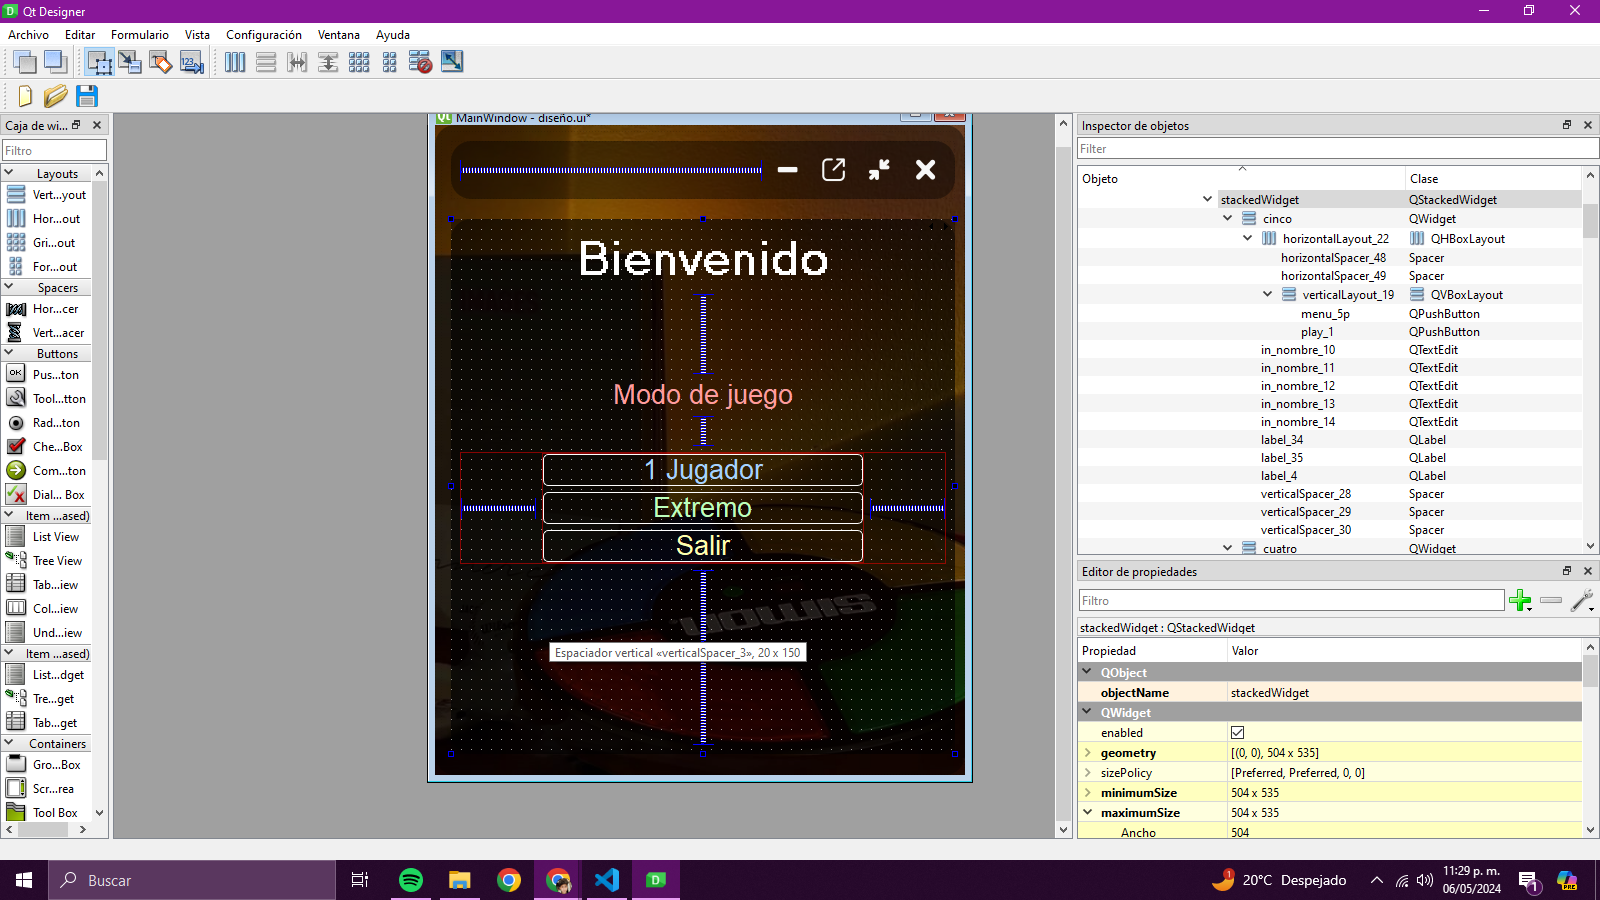
\includegraphics[width=1\textwidth]{Captura de pantalla (754).png} 


\end{figure}

\vspace{.5\baselineskip}




\newpage 
\vspace{0.2cm}
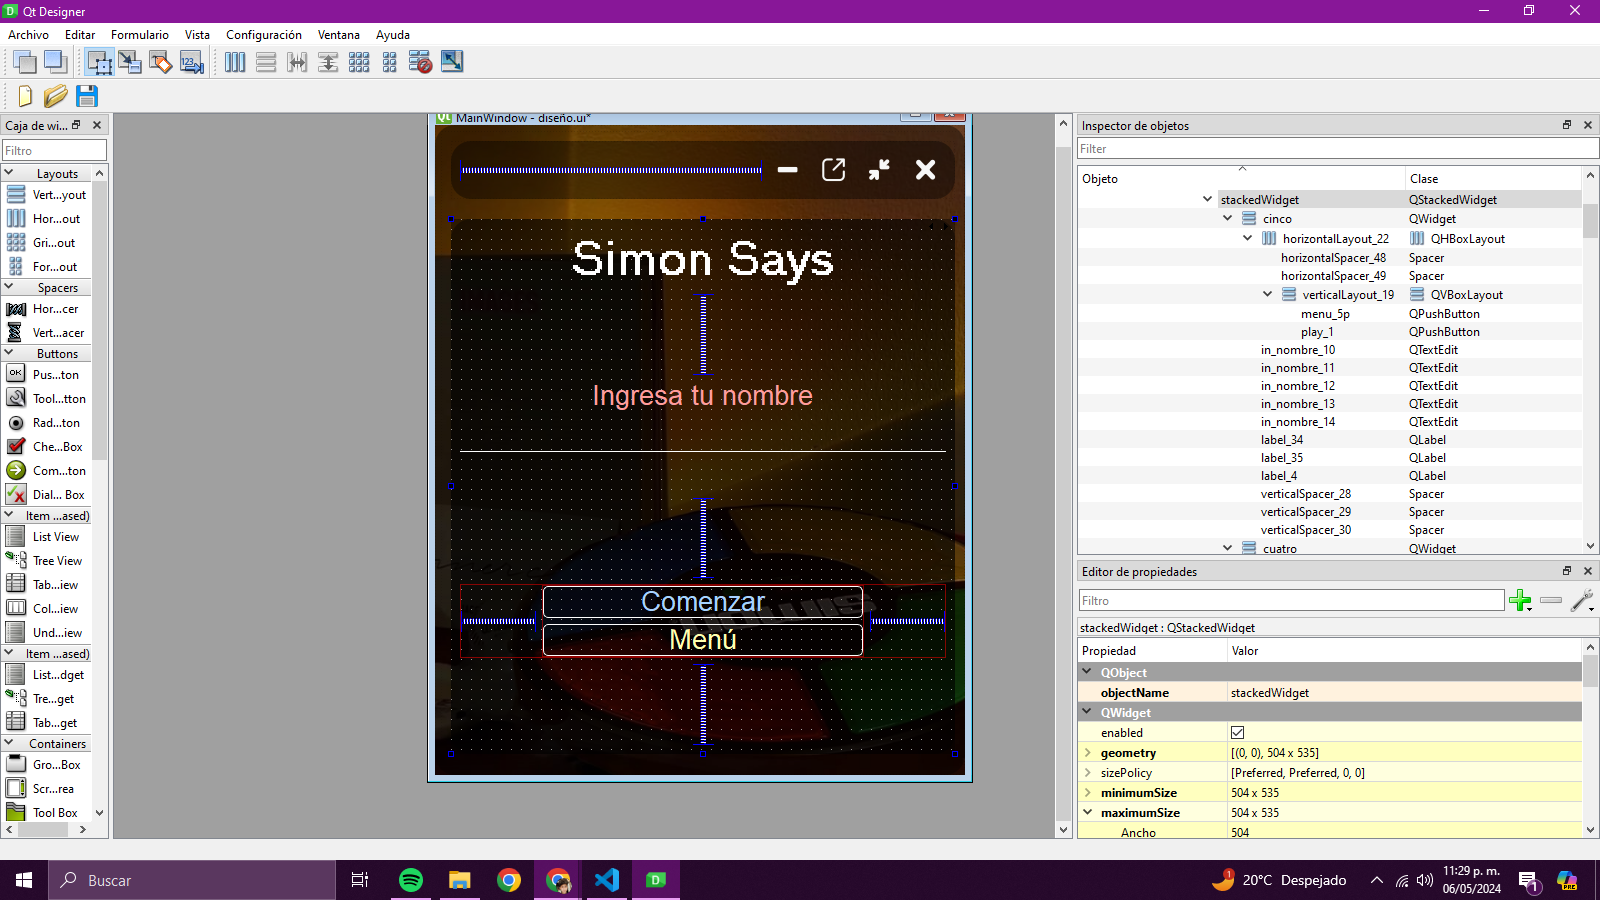
\includegraphics[width=1\linewidth]{Captura de pantalla (755).png}

\vspace{0.2cm}


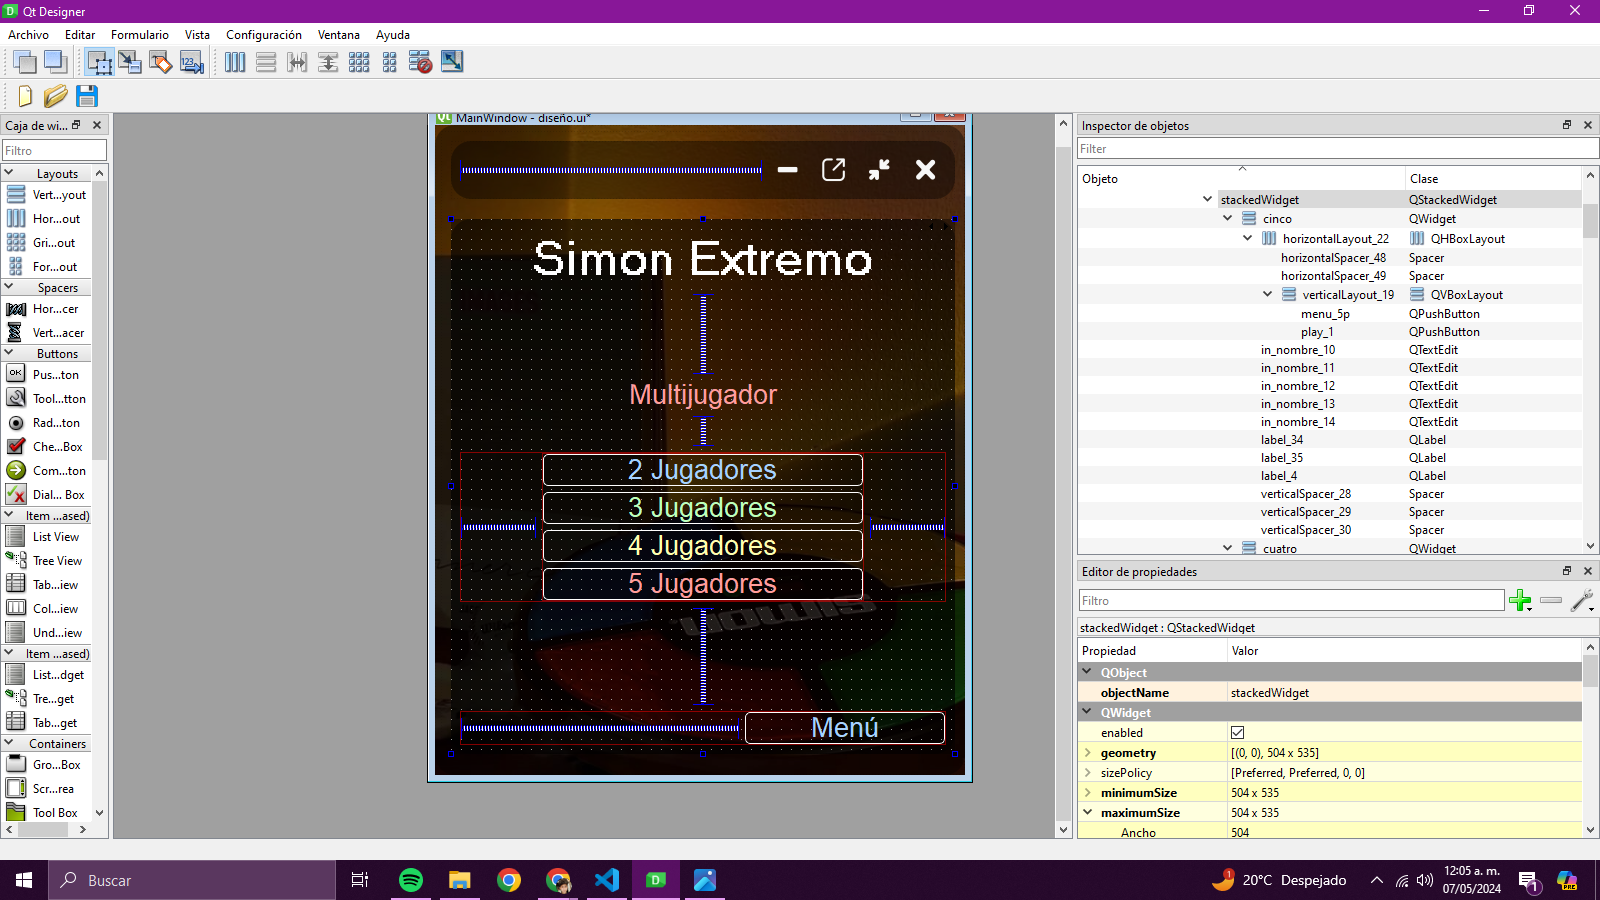
\includegraphics[width=1\linewidth]{Captura de pantalla (756).png}

\vspace{0.2cm}
{\Large \\ El stackWidget de simon says es para la modalidad de un solo jugador, la cual permite al usuario registrar su nombre y poder comenzar o regresar al menu, pero no funcionara hasta que se le ponga play en la siguiente pagina de ese StackWidget

} 


\newpage

\vspace{0.2cm}
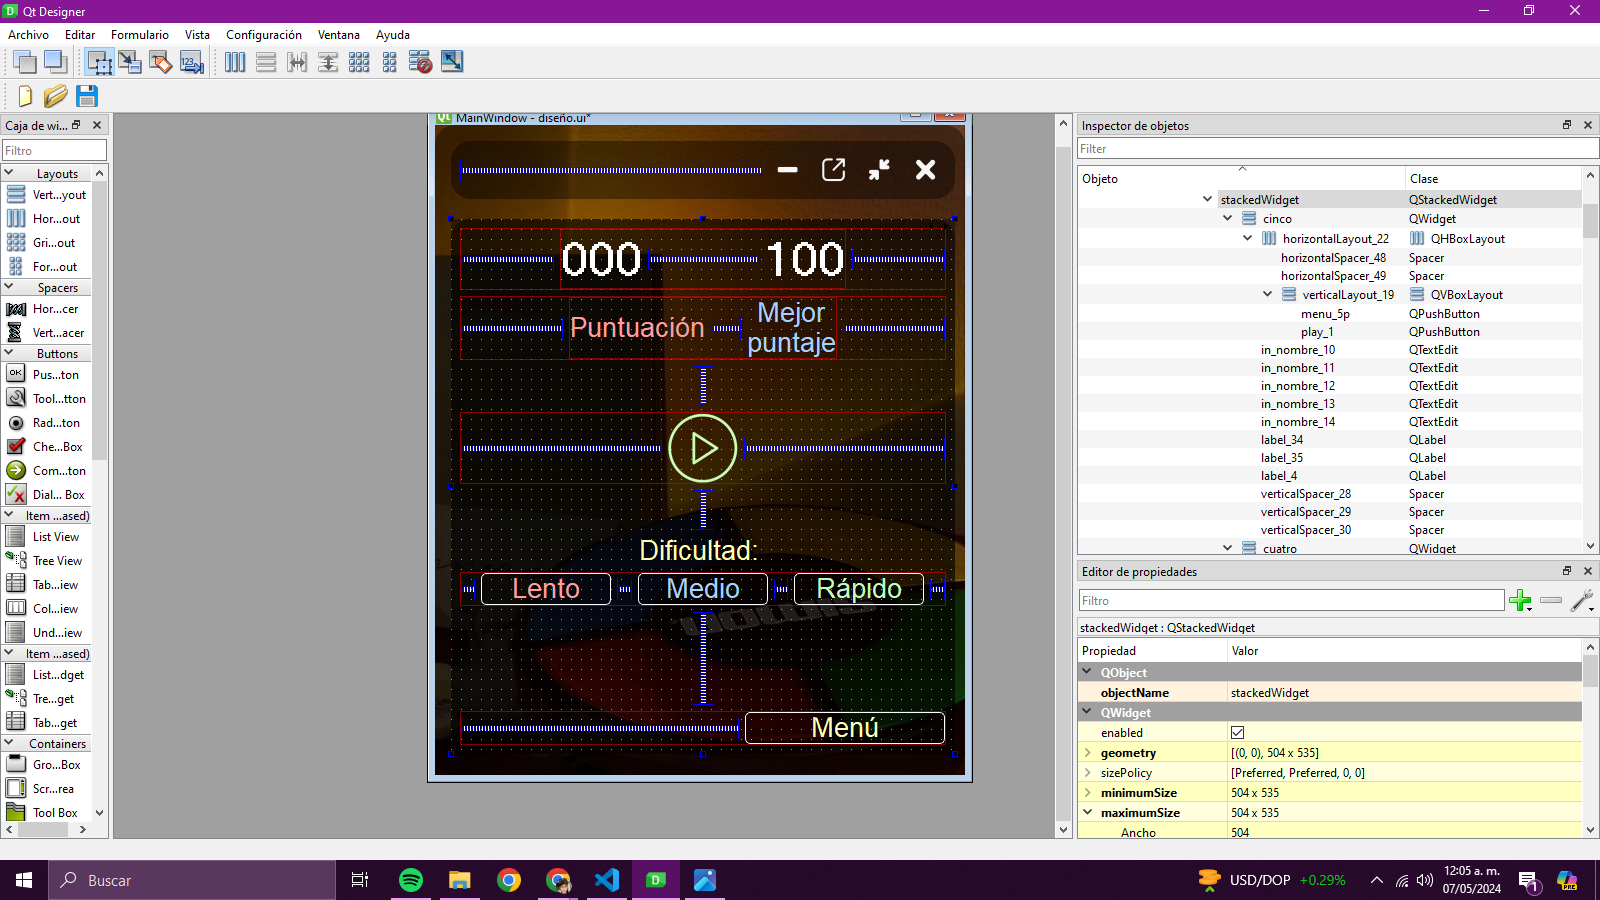
\includegraphics[width=1\linewidth]{Captura de pantalla (757).png}

\vspace{0.2cm}


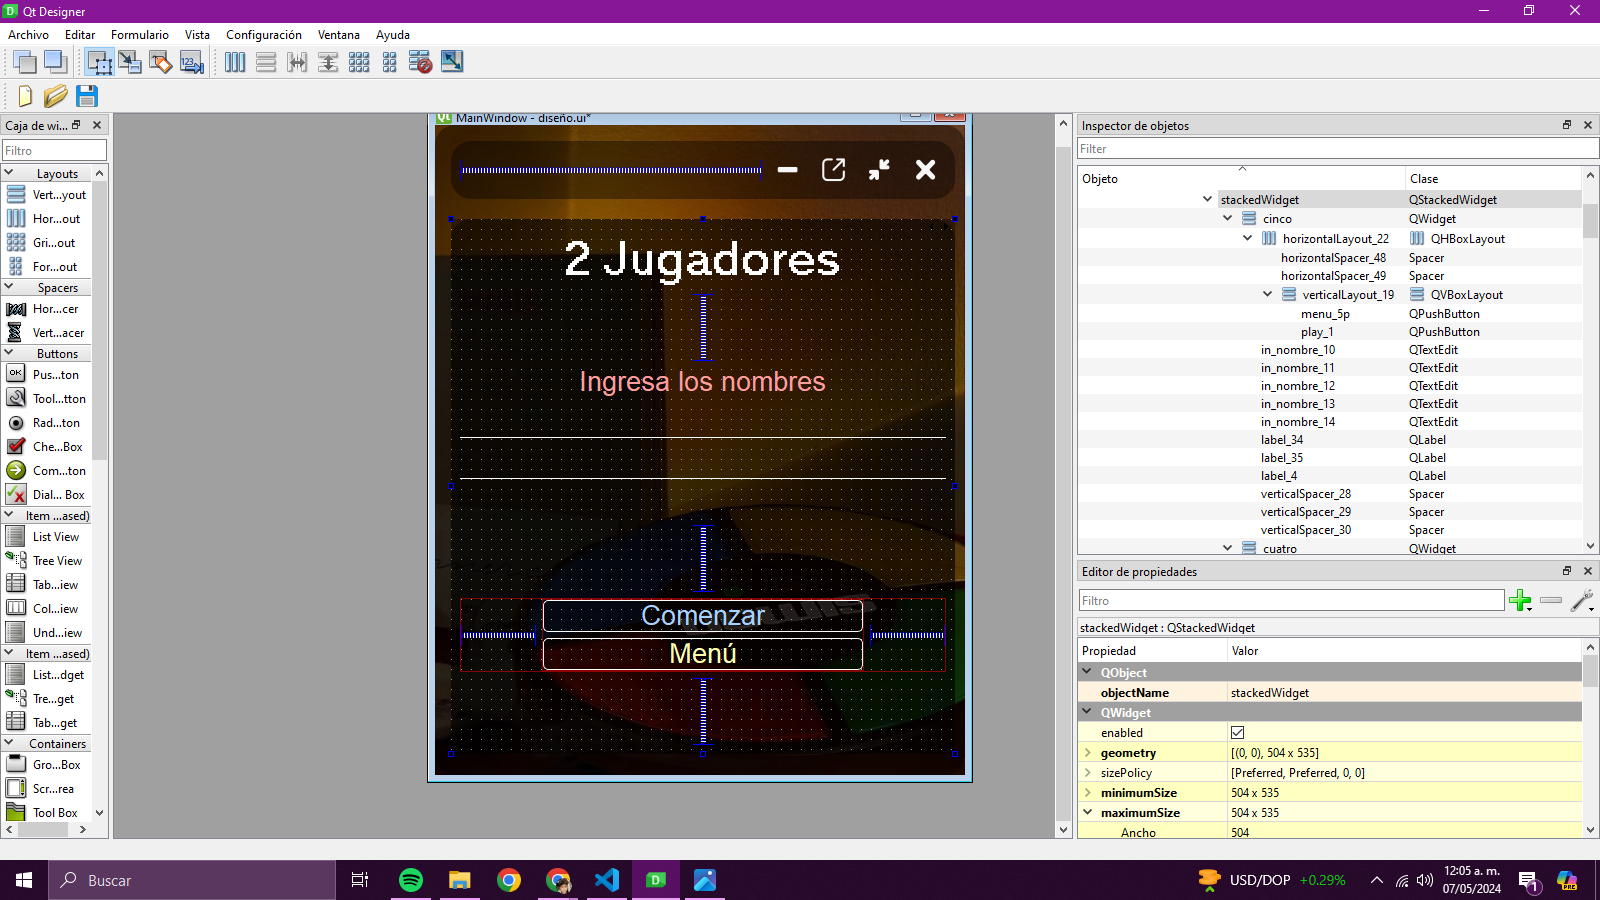
\includegraphics[width=1\linewidth]{Captura de pantalla (758).png}

\vspace{0.2cm}

{\Large La pagina de la puntuacion basicamente es la segunda principal, ya que nos indica el mejor puntaje , iniciar el juego poniendole play y la dificultad del juego 
 \\En la otra pagina tenemos la version de multijugador de 2 jugadores }




\newpage
\vspace{0.2cm}
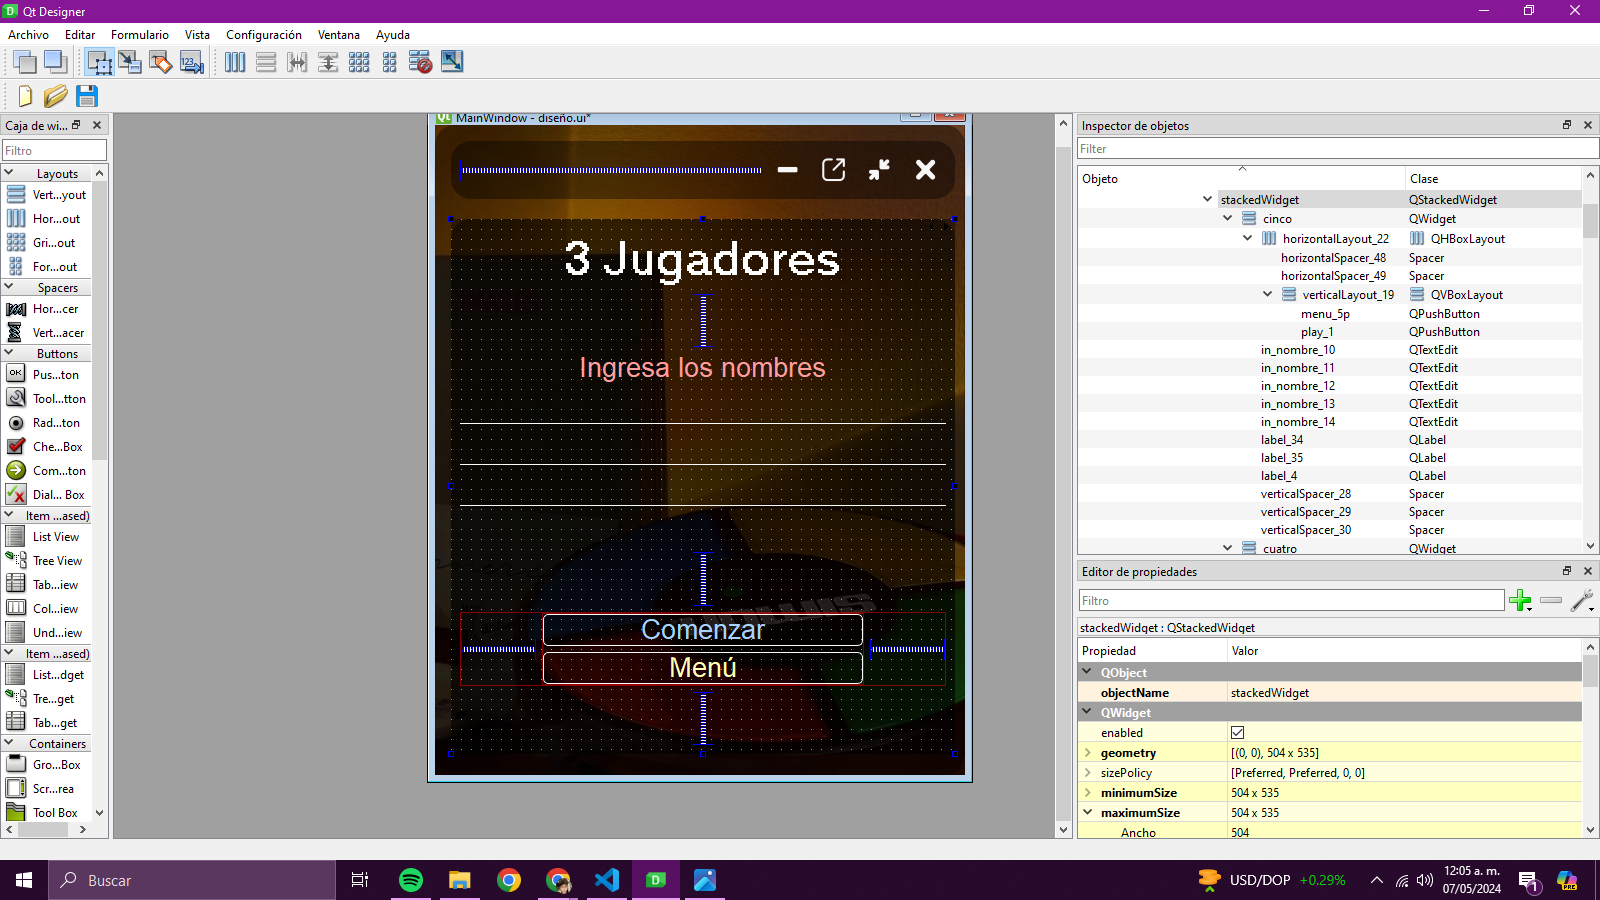
\includegraphics[width=1\linewidth]{Captura de pantalla (759).png}

\vspace{0.2cm}


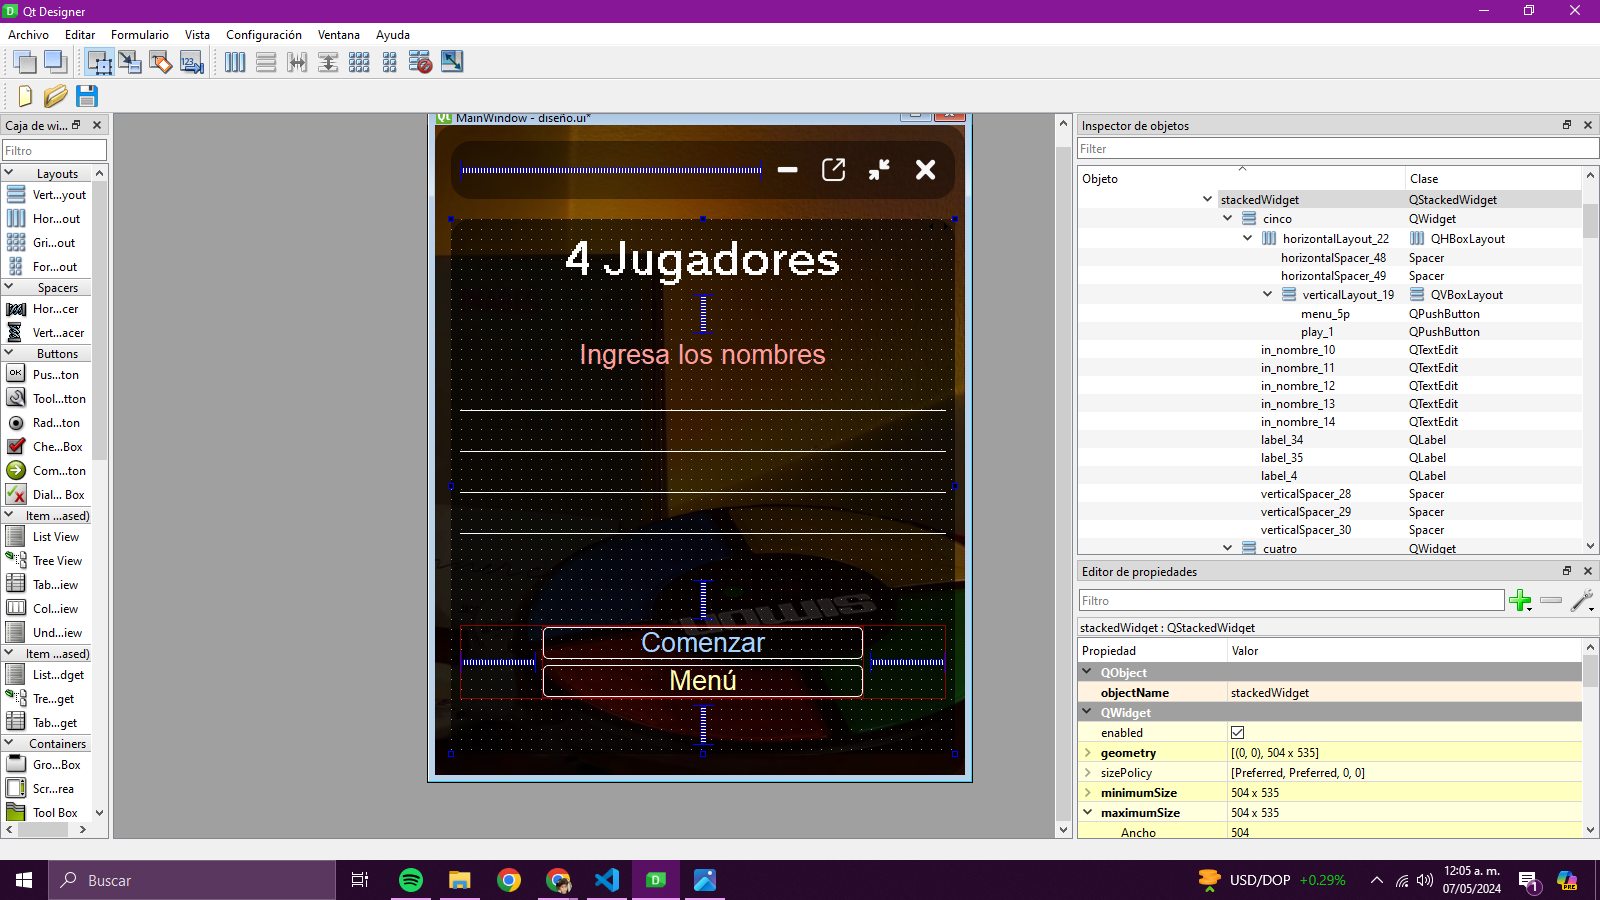
\includegraphics[width=1\linewidth]{Captura de pantalla (760).png}

\vspace{0.2cm}


{\Large Aqui se pueden observar las paginas para 3 y 4 jugadores, donde nos pide en cada una que registremos los nombres de los respectivos numeros de jugadores, aparte de que despues nos sacara a la pagina de play para comenzar el juego, cuando obviamente presionemos el boton comenzar, menu nos volvera al inicio, recordemos que para que exista un perdedor, simplemente al equivocarse en la secuencia podremos eleminar a cada uno y asi sucesivamente hasta que prevalezca uno\\ }



\newpage


\vspace{0.2cm}
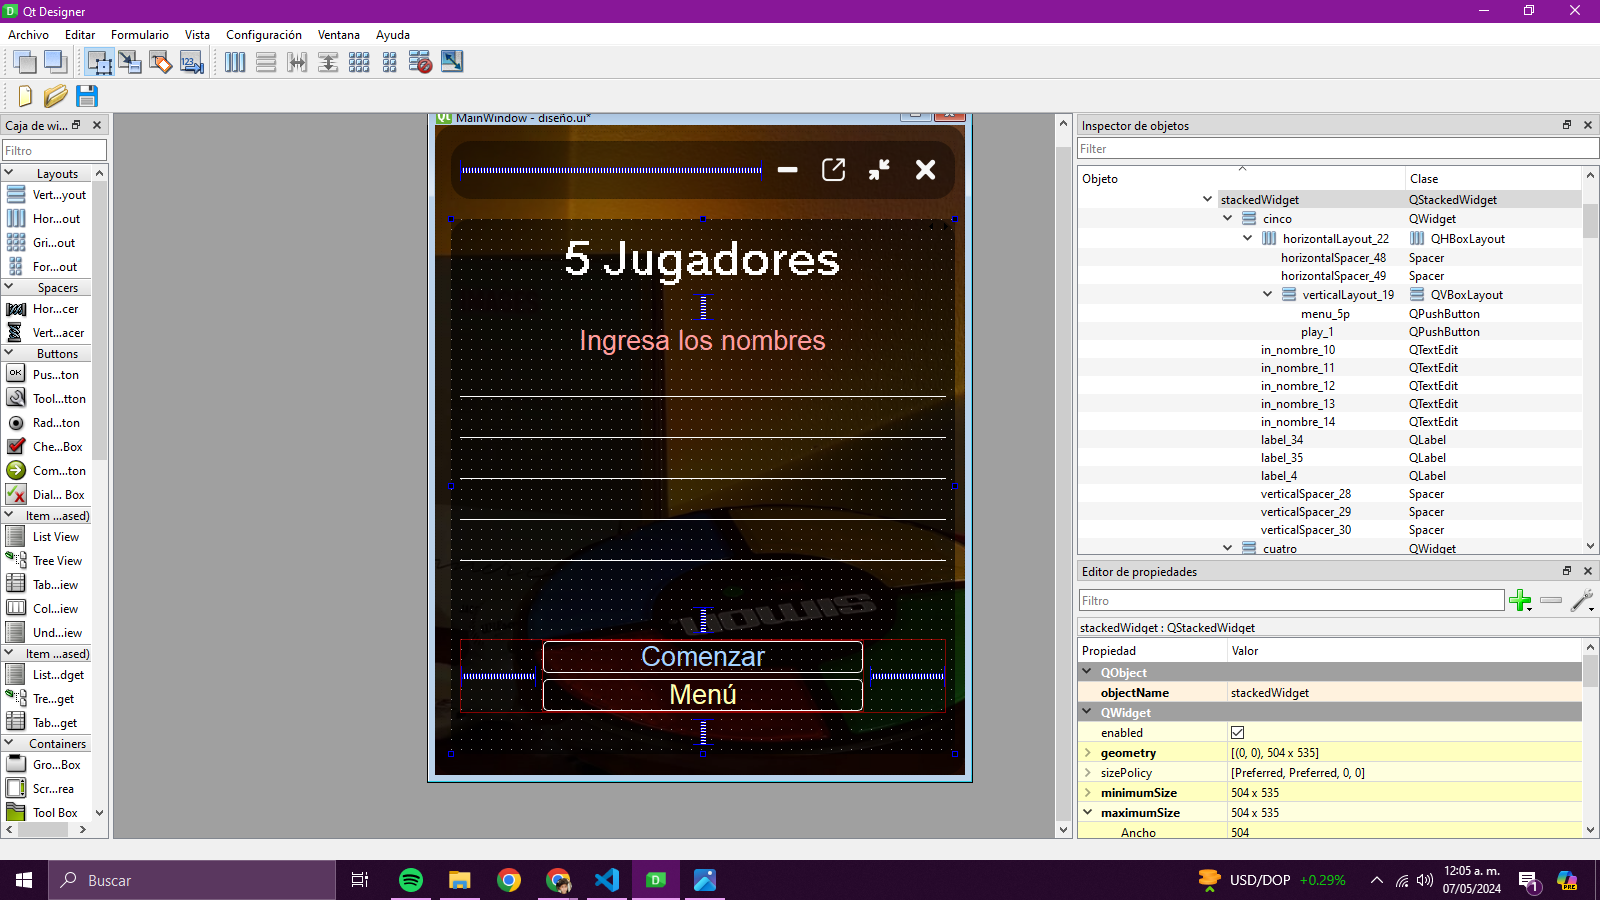
\includegraphics[width=0.8\linewidth]{Captura de pantalla (761).png}

\vspace{0.2cm}


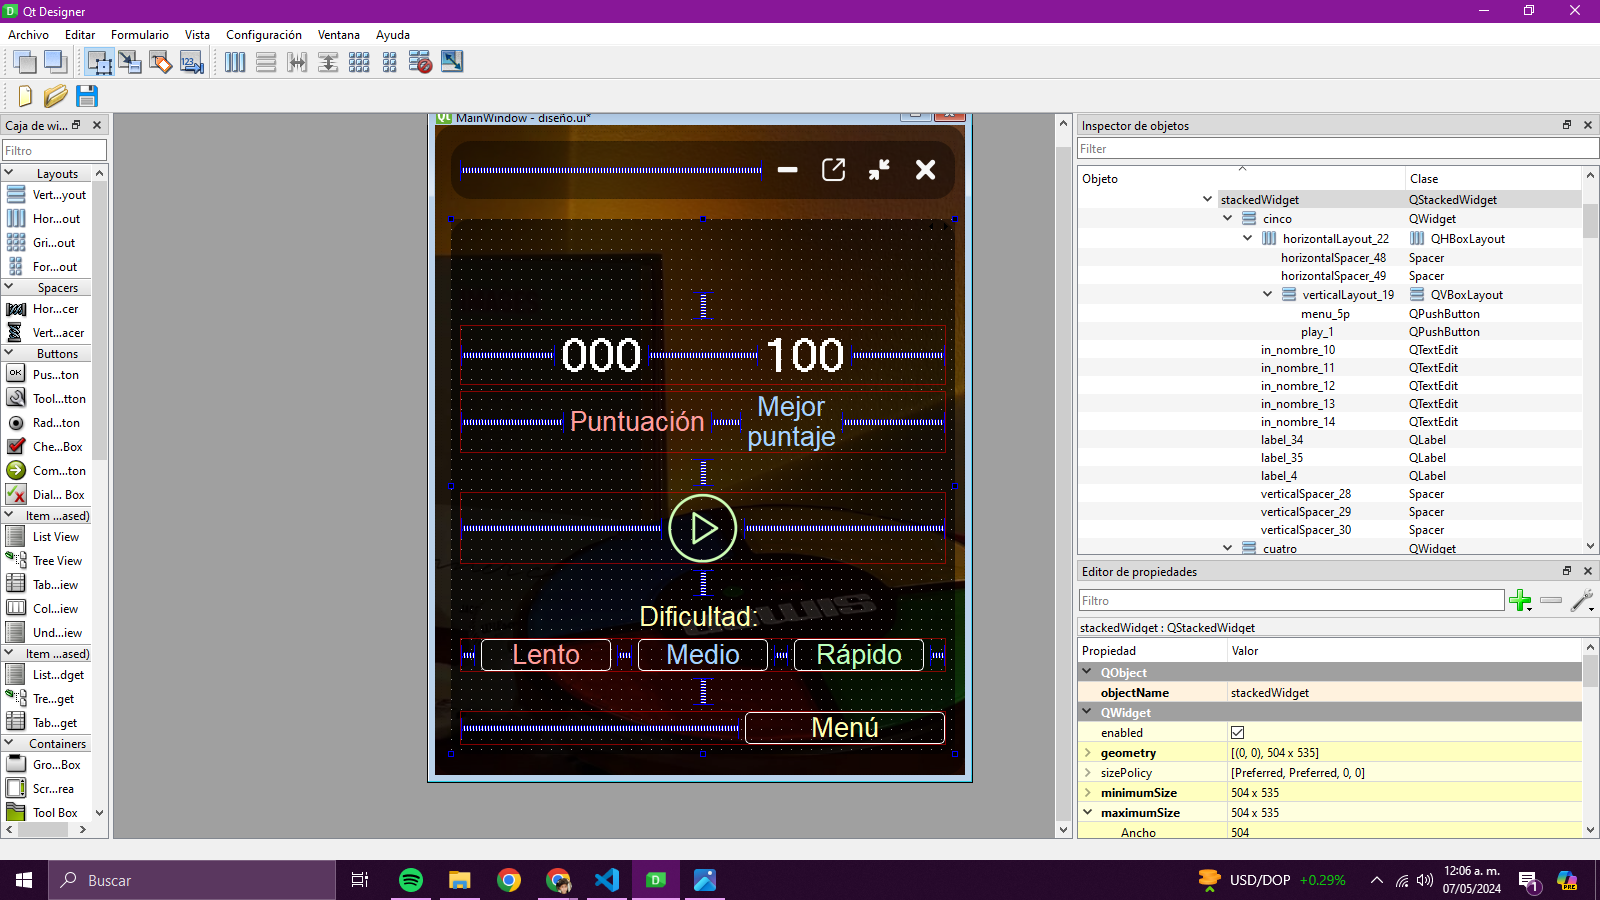
\includegraphics[width=0.8\linewidth]{Captura de pantalla (762).png}

\vspace{0.2cm}

{\Large \\ Tenemos nuevamente el modo multijugador pero en esta ocasion para 5 personas, con los mismo botones que las paginas antoeriores, simplemente que aqui nos pedira los nombres de los 5 participantes. Y finalmente le damos la vuelta para que las pagianas nos muestren los resultados y el puntaje mas alto registrado.  Cabe destacar que el servo quirara hacia el lado del jugador que le toque, como solo son 180 grados, por lo tanto seran esos 180 sobre el numero de jugadores que estan. 





\newpage

{\Large De nuestro lado izquierdo inferior podemos observar la ultima pagina, las cual nos dice los puntajes y demas valores para cuando se juega extremo (multijugador)\\
Del lado derecho podemos observar el diagrama de nuestro circuito en arduino, obviamente con mas botones y leds. pero es la misma funcionalidad, se prende un led, usted o el jugador debera de presionarlo para que la secuencia que se mando al arduino , sea la misma y de esa manera no pierda tal jugador y asi sucesivamente

\begin{figure}[h]            
    \begin{minipage}{0.55\textwidth}  
        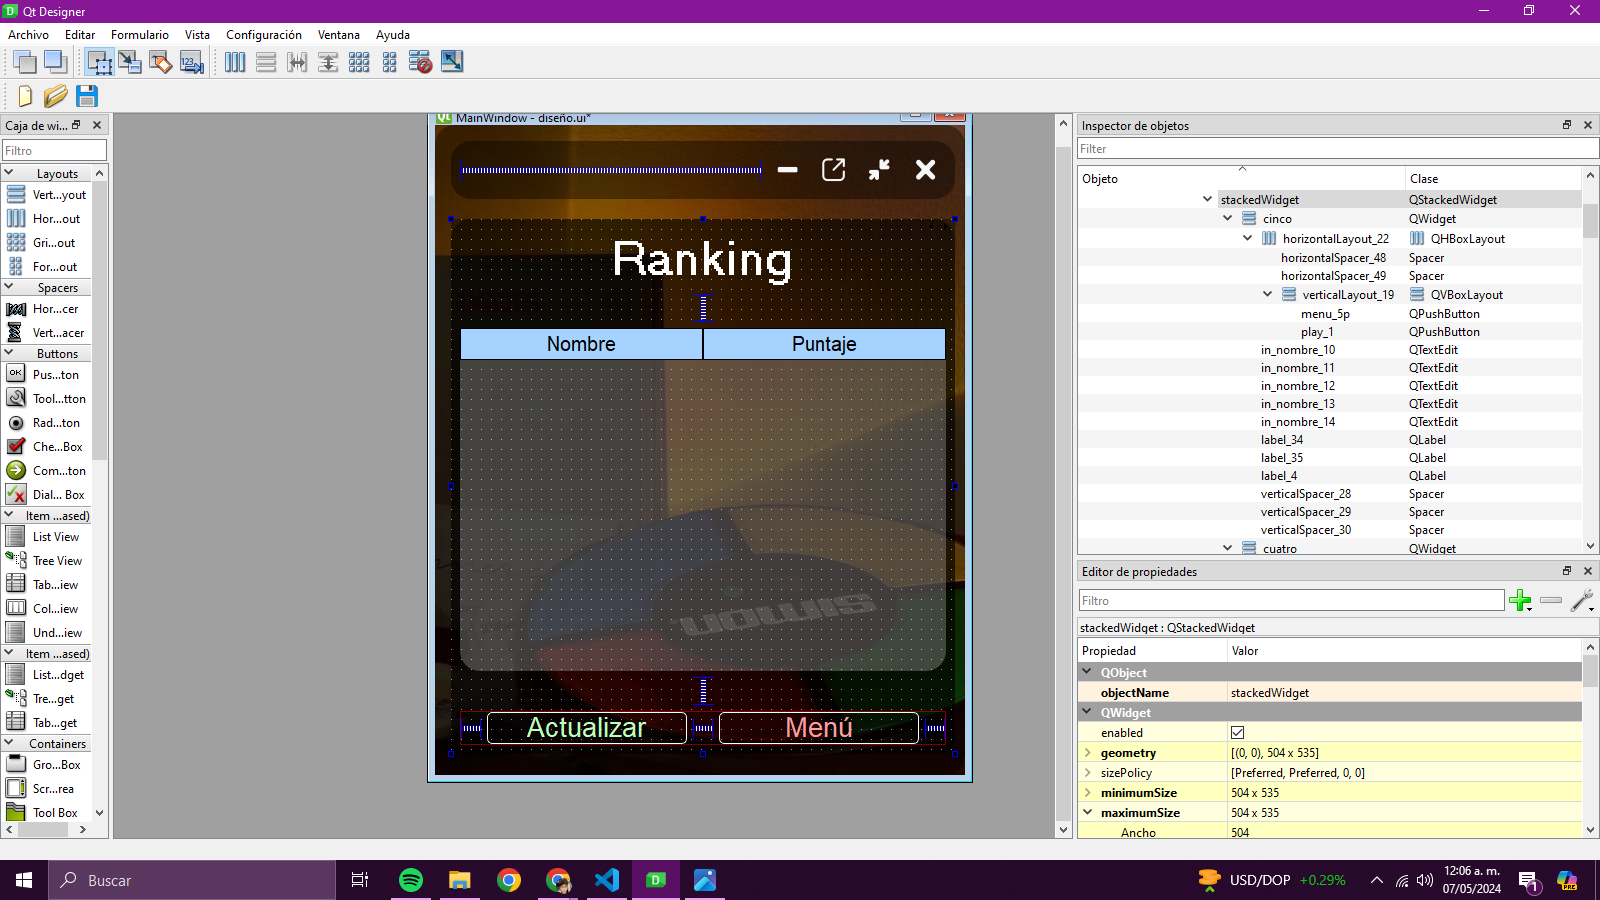
\includegraphics[width=\textwidth]{Captura de pantalla (763).png}
    \end{minipage}
    \hfill
    \begin{minipage}{0.5\textwidth}
        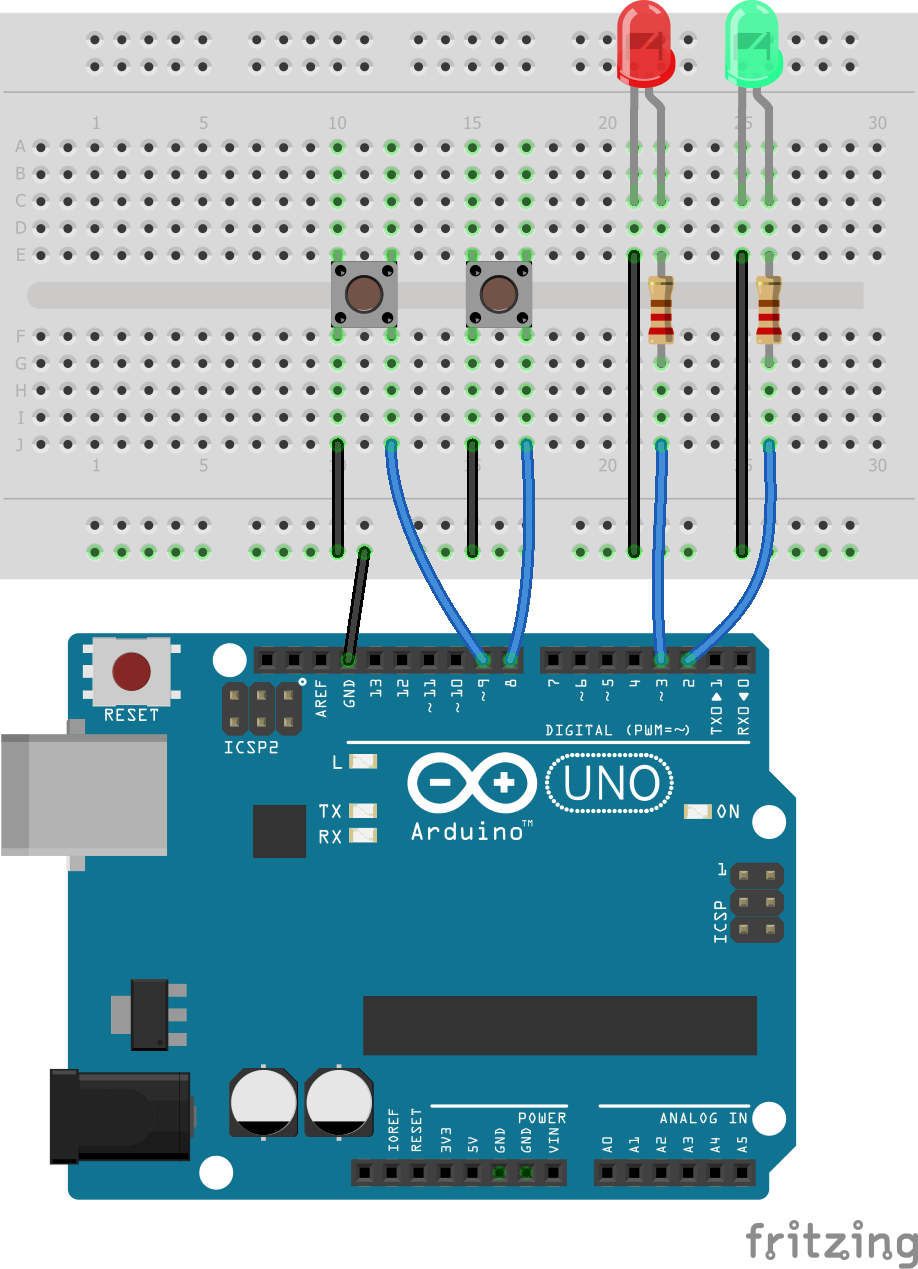
\includegraphics[width=\textwidth]{arduino-proto-04-push-ledes-bb.png}
    \end{minipage}
    
\end{figure}






\newpage
\begin{figure}[h]
    \centering
    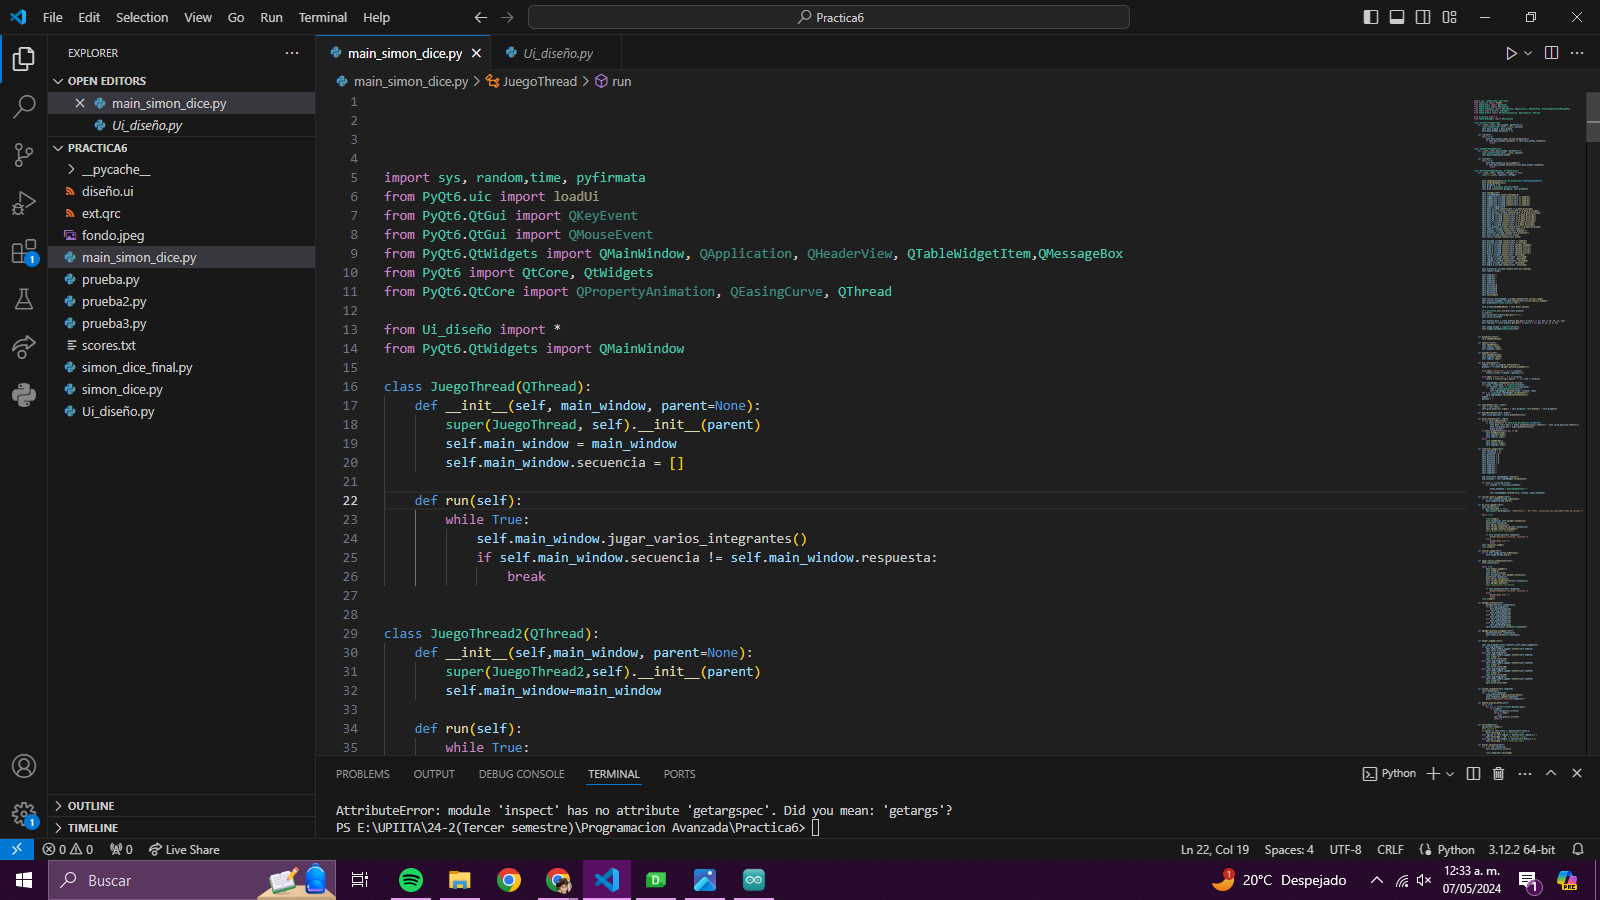
\includegraphics[width=1\textwidth]{Captura de pantalla (764).png}
    
\end{figure}

{\Large \\JuegoThread maneja el juego con múltiples jugadores, mientras que JuegoThread2 se encarga del juego para un solo jugador. Ambos subprocesos ejecutan un bucle infinito donde llaman a métodos específicos del objeto mainwindow, como jugarvariosintegrantes() o unsolojugador(), para gestionar la lógica del juego. Estos subprocesos se detienen cuando la secuencia generada por mainwindow no coincide con la respuesta esperada, indicando un error en el juego.

}

\newpage
\begin{figure}[h]
    \centering
    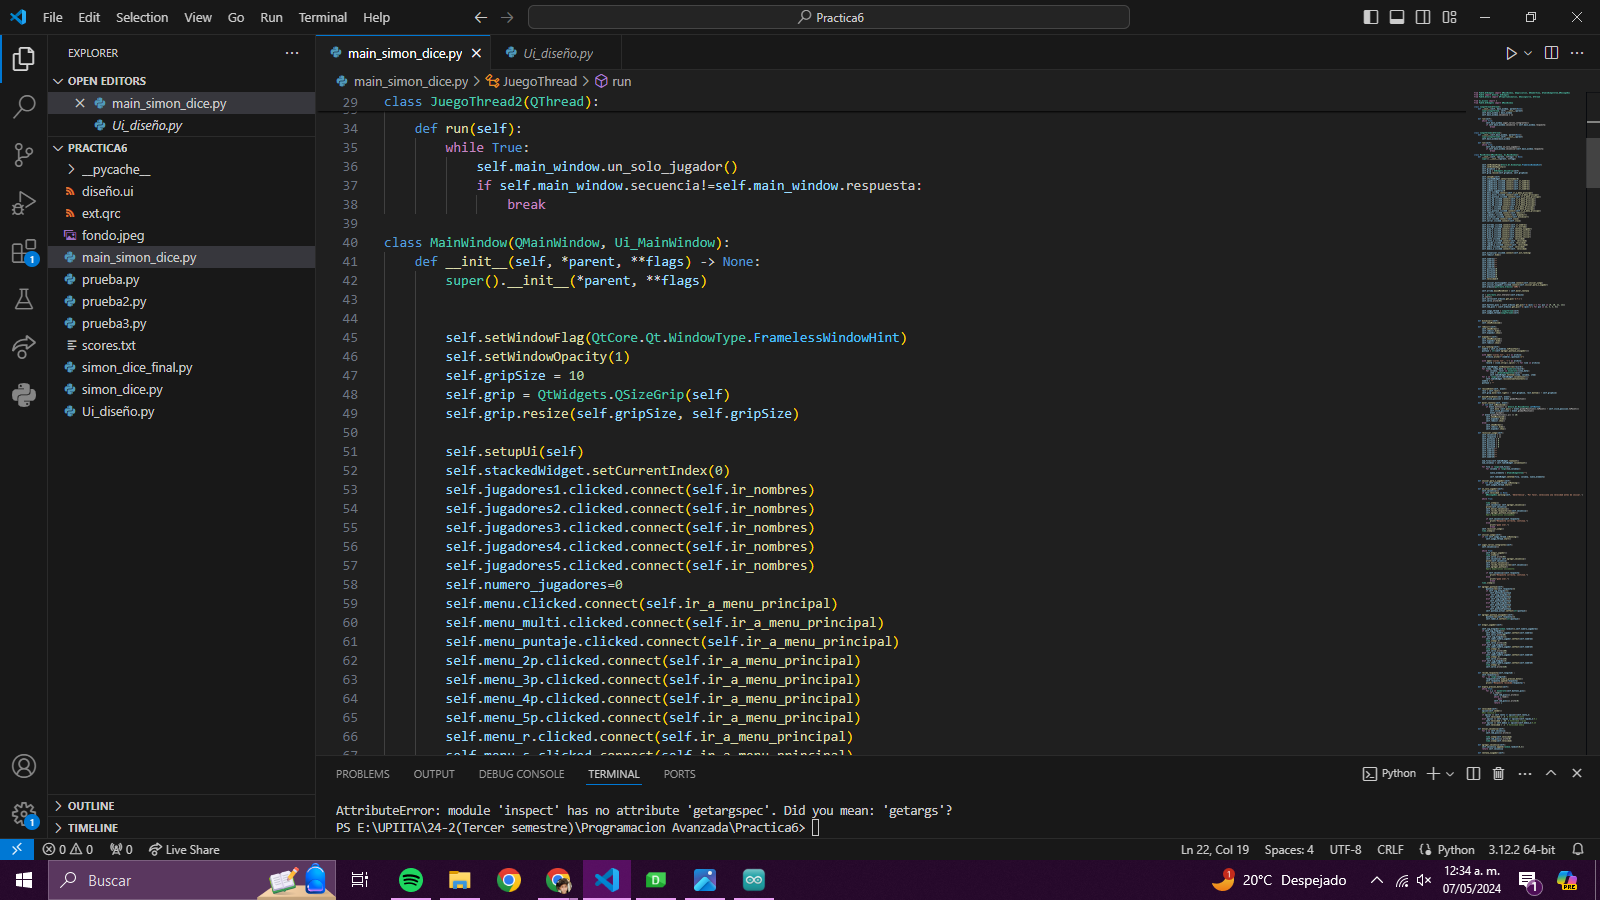
\includegraphics[width=1\textwidth]{Captura de pantalla (765).png}
    
\end{figure}

{\Large Establecemos la ventana principal de la aplicación y define su interfaz de usuario. Configura la ventana sin bordes y con una opacidad completa. Luego, carga la interfaz de usuario desde un archivo externo y configura los botones para realizar diferentes acciones, como cambiar entre menús o iniciar juegos. Además, maneja eventos como minimizar, expandir o cerrar la ventana. También inicializa variables para almacenar nombres y puntajes de jugadores, junto con la velocidad del juego. Finalmente, conecta señales de otros widgets a funciones que realizan diversas acciones, como actualizar el ranking o iniciar juegos multijugador

}

\newpage
\begin{figure}[h]
    \centering
    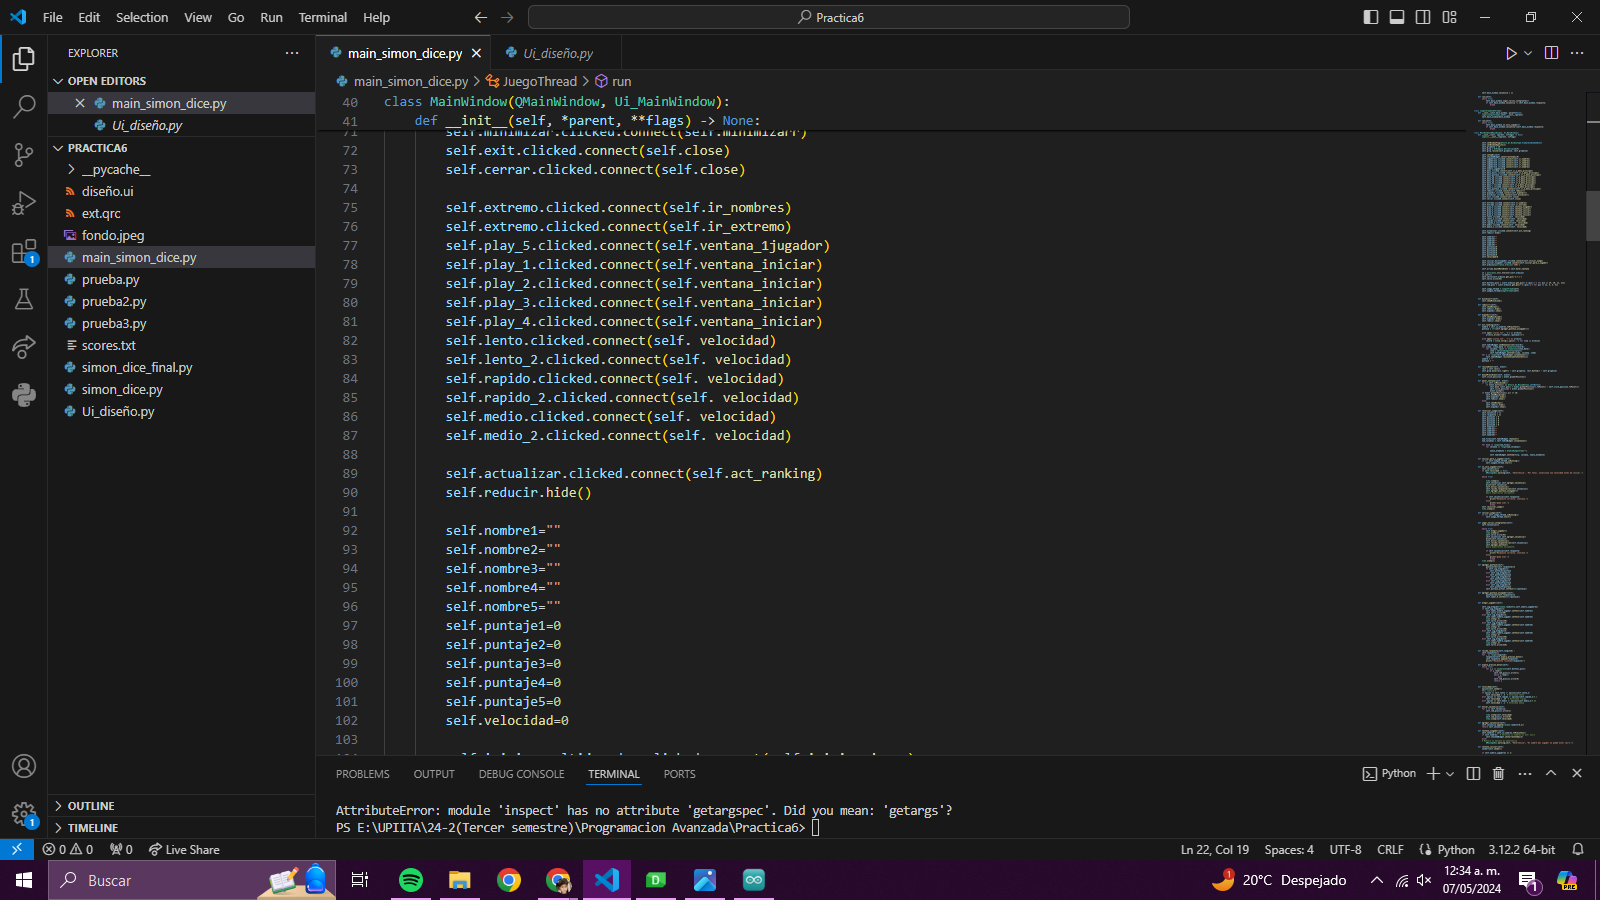
\includegraphics[width=1\textwidth]{Captura de pantalla (766).png}
    
\end{figure}

{\Large De igual  manera seguimos conectando botones a la interfaz

}


\newpage
\begin{figure}[h]
    \centering
    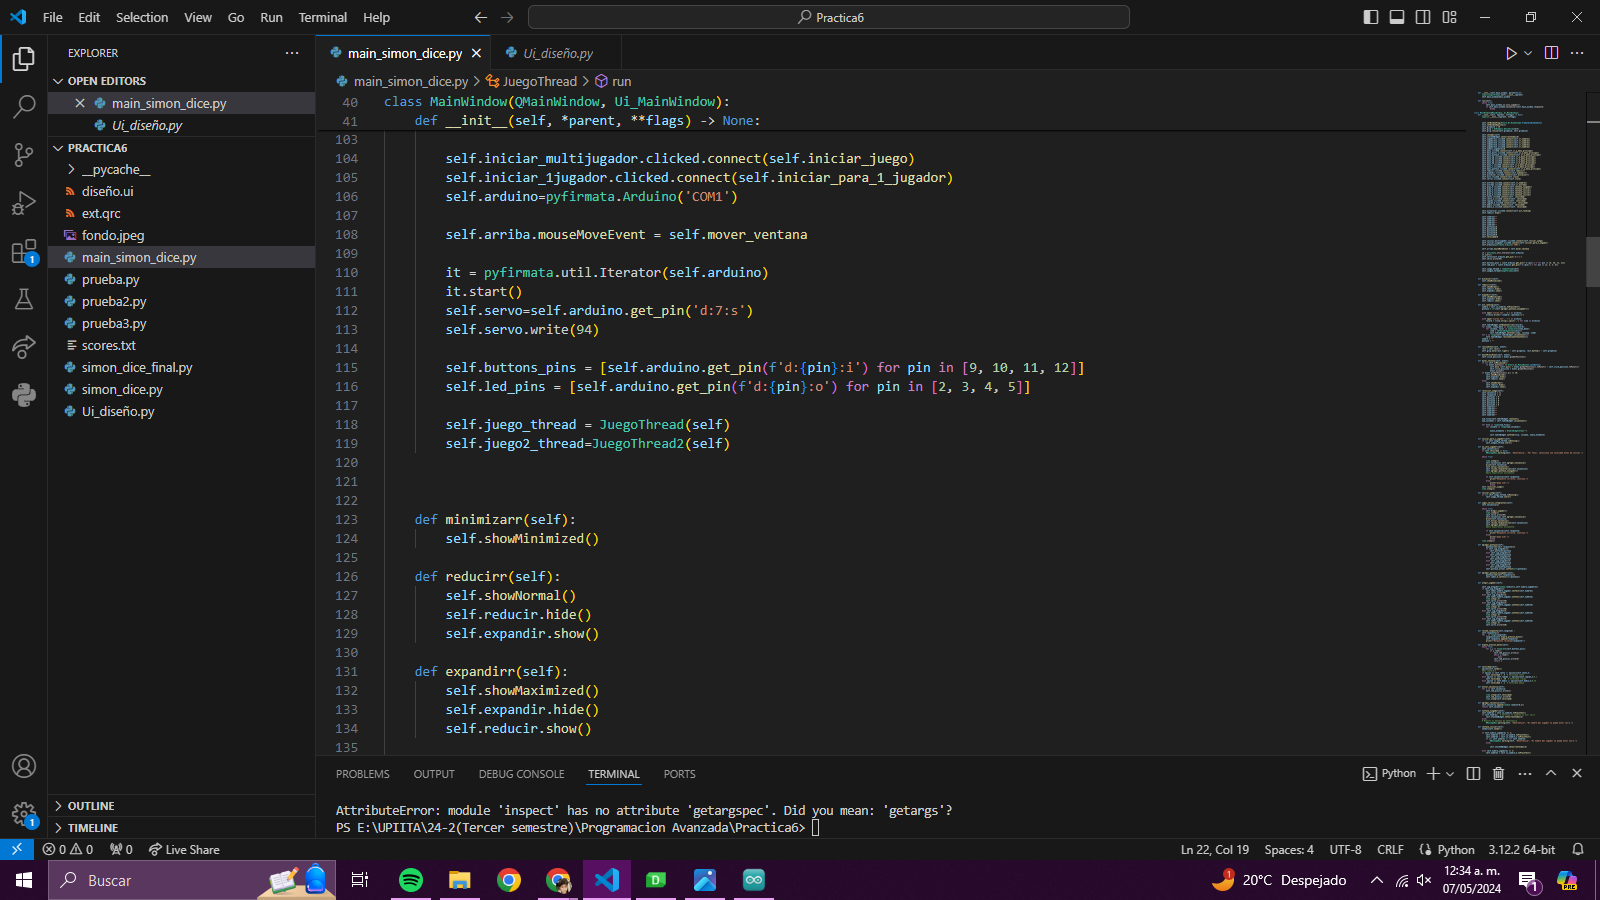
\includegraphics[width=1\textwidth]{Captura de pantalla (767).png}
    
\end{figure}

{\Large conecta las señales emitidas por los botones iniciarmultijugador e iniciar1jugador a las funciones iniciarjuego e iniciarpara1jugador, respectivamente. Además, inicializa la comunicación con un dispositivo Arduino conectado al puerto COM1. Configura el movimiento de la ventana a través del evento mouseMoveEvent y comienza un iterador para comunicarse con la placa Arduino. Luego, inicializa los pines de entrada y salida del Arduino para controlar botones y LEDs. Finalmente, crea instancias de las clases JuegoThread y JuegoThread2 para manejar los hilos del juego. Las funciones minimizarr, reducirr y expandirr controlan el comportamiento de la ventana cuando se minimiza, reduce o expande, respectivamente

}

\newpage
\begin{figure}[h]
    \centering
    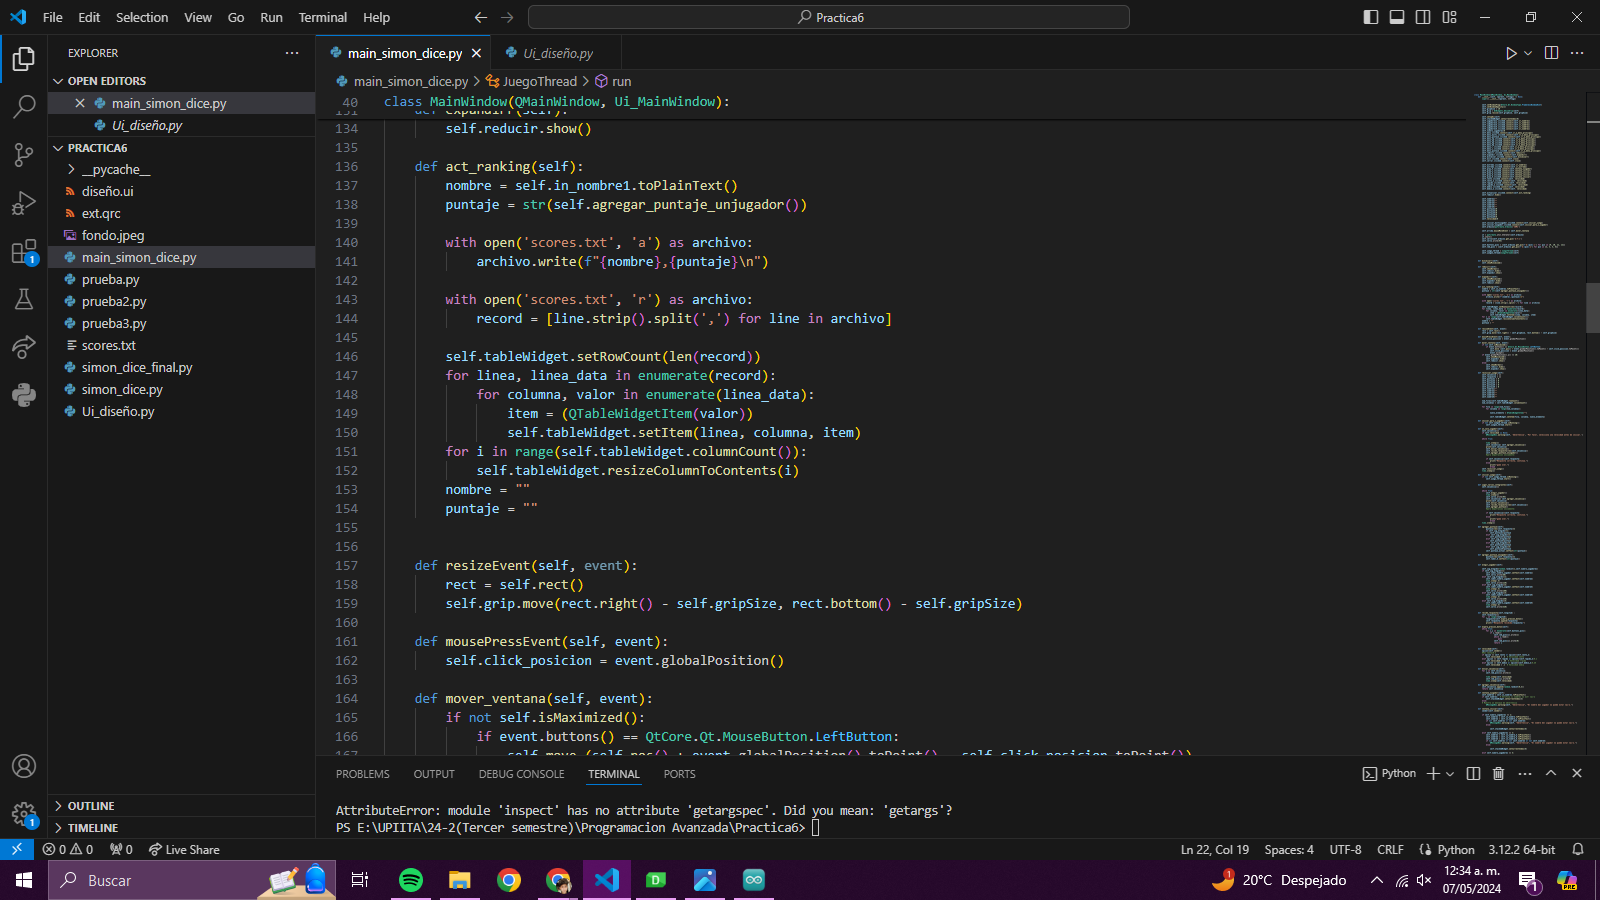
\includegraphics[width=1\textwidth]{Captura de pantalla (768).png}
    
\end{figure}

{\Large La función actranking actualiza el registro de puntajes en un archivo de texto. Primero, toma el nombre ingresado por el usuario y el puntaje actual. Luego, escribe esta información en un archivo llamado 'scores.txt'. Después, lee el contenido de este archivo y lo muestra en una tabla para que el usuario pueda ver el ranking actualizado. Las otras funciones (resizeEvent, mousePressEvent, moverventana) están relacionadas con la manipulación y el comportamiento de la ventana
}

\newpage
\begin{figure}[h]
    \centering
    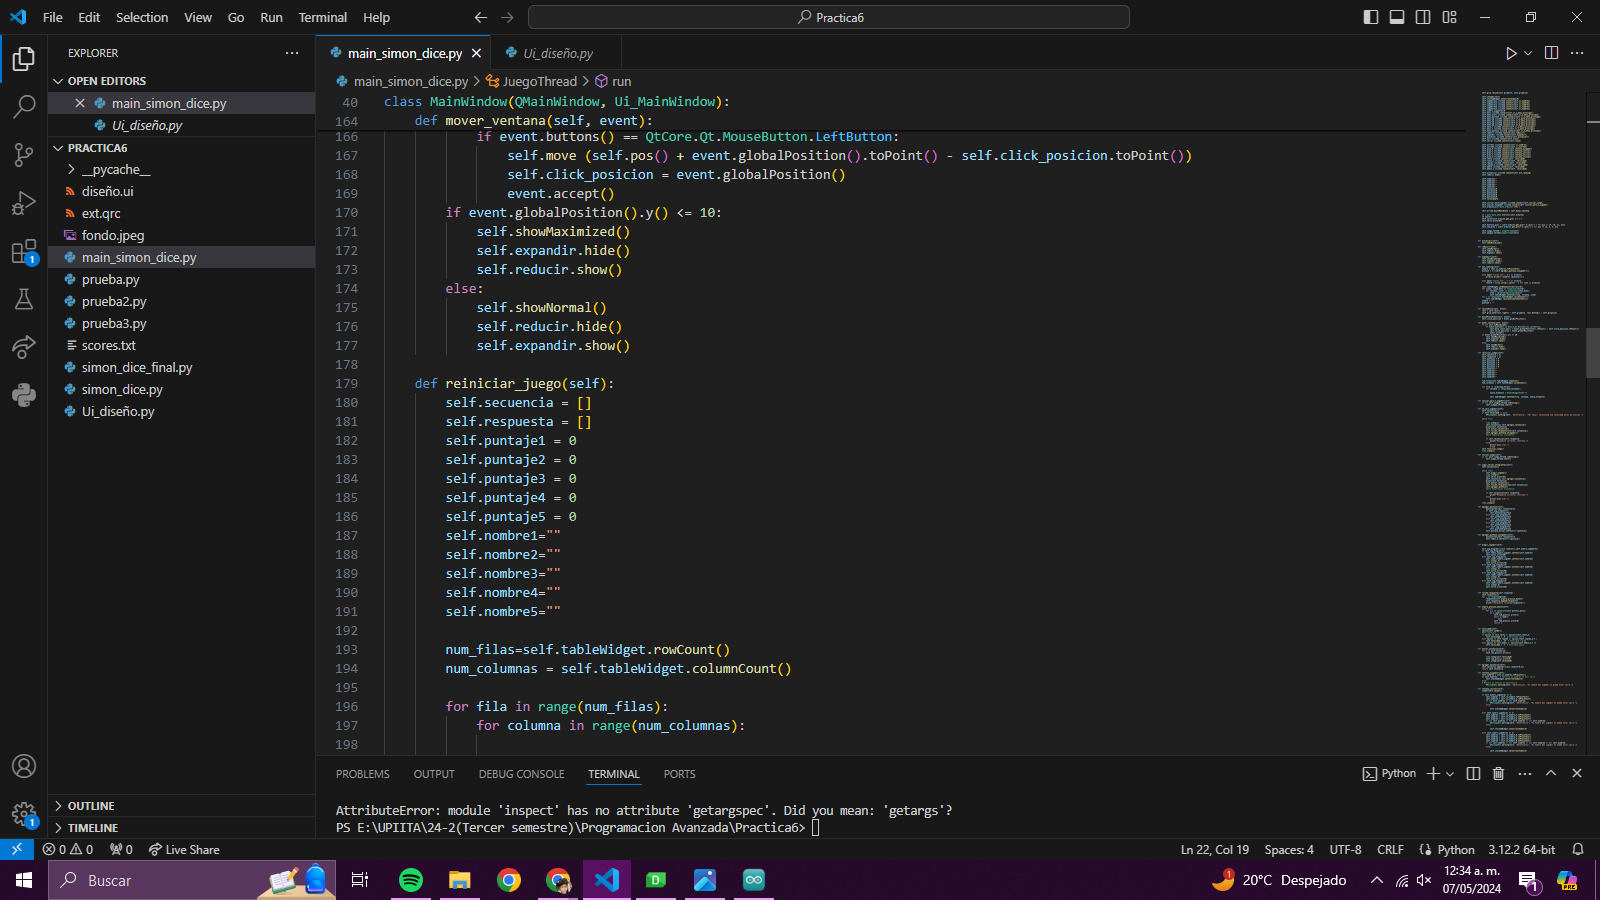
\includegraphics[width=1\textwidth]{Captura de pantalla (769).png}
    
\end{figure}

{\Large La función `iniciarpara1jugador` inicia el juego para un solo jugador si el hilo correspondiente no está en ejecución.

La función `unsolojugador` ejecuta el juego para un solo jugador, donde se genera una secuencia de juego, se envía al jugador, se espera su respuesta, se actualiza el puntaje y se verifica si la respuesta es correcta. Si la respuesta es incorrecta, el juego se detiene y se reinicia.

}



\newpage
\begin{figure}[h]
    \centering
    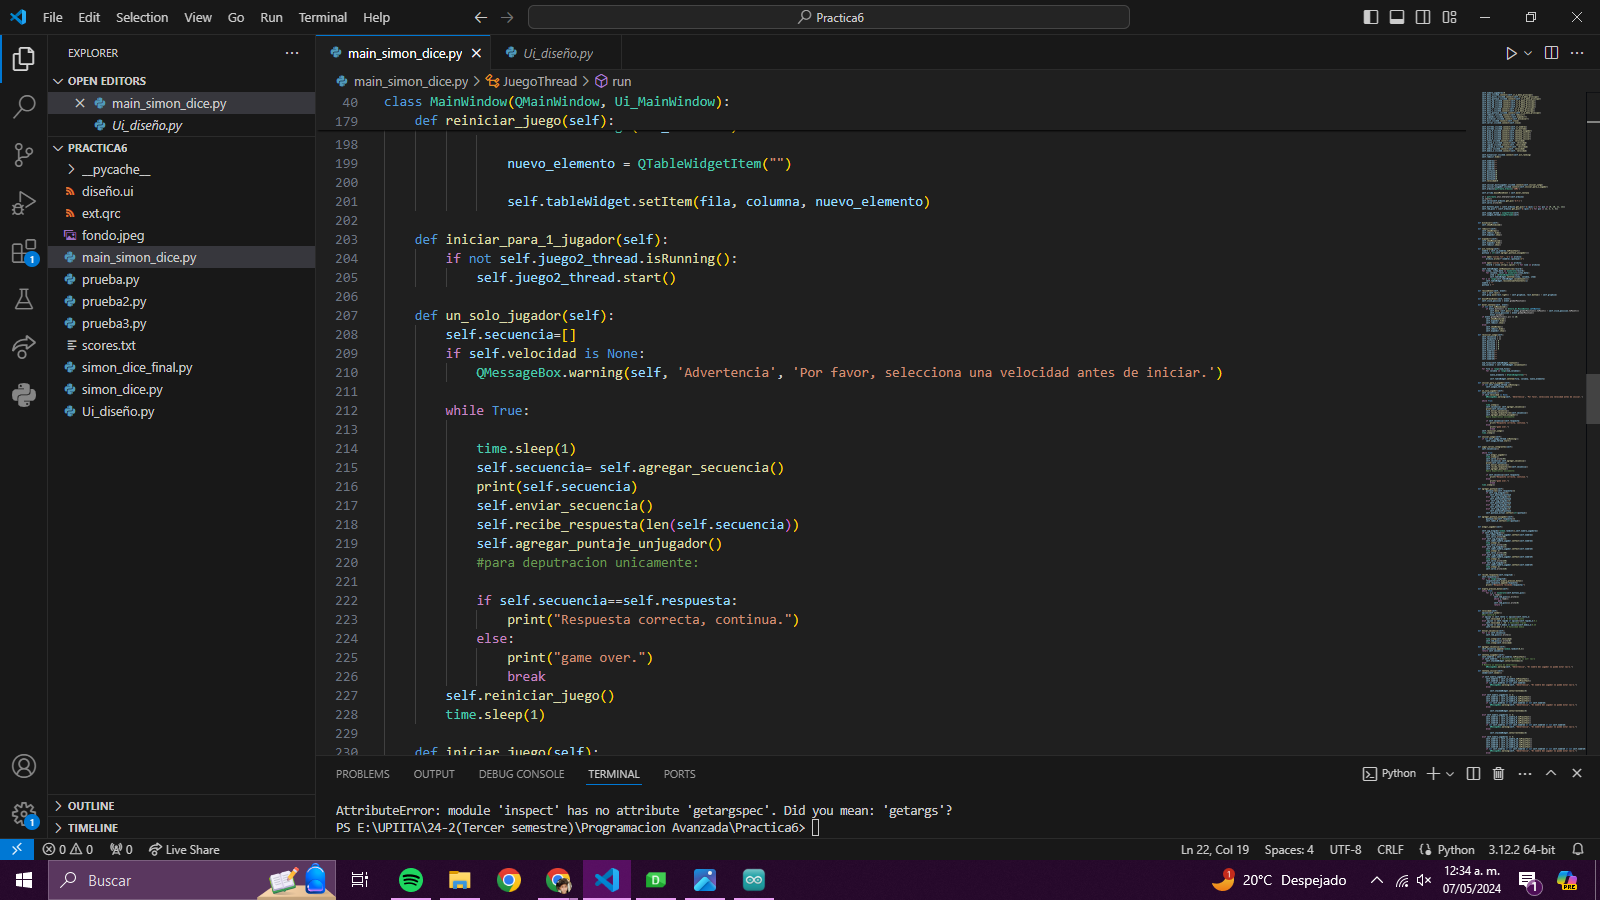
\includegraphics[width=1\textwidth]{Captura de pantalla (770).png}
    
\end{figure}

{\Large La función `iniciarpara1jugador` inicia el juego para un solo jugador si el hilo correspondiente no está en ejecución.

La función `unsolojugador` ejecuta el juego para un solo jugador, donde se genera una secuencia de juego, se envía al jugador, se espera su respuesta, se actualiza el puntaje y se verifica si la respuesta es correcta. Si la respuesta es incorrecta, el juego se detiene y se reinicia.

}




\newpage
\begin{figure}[h]
    \centering
    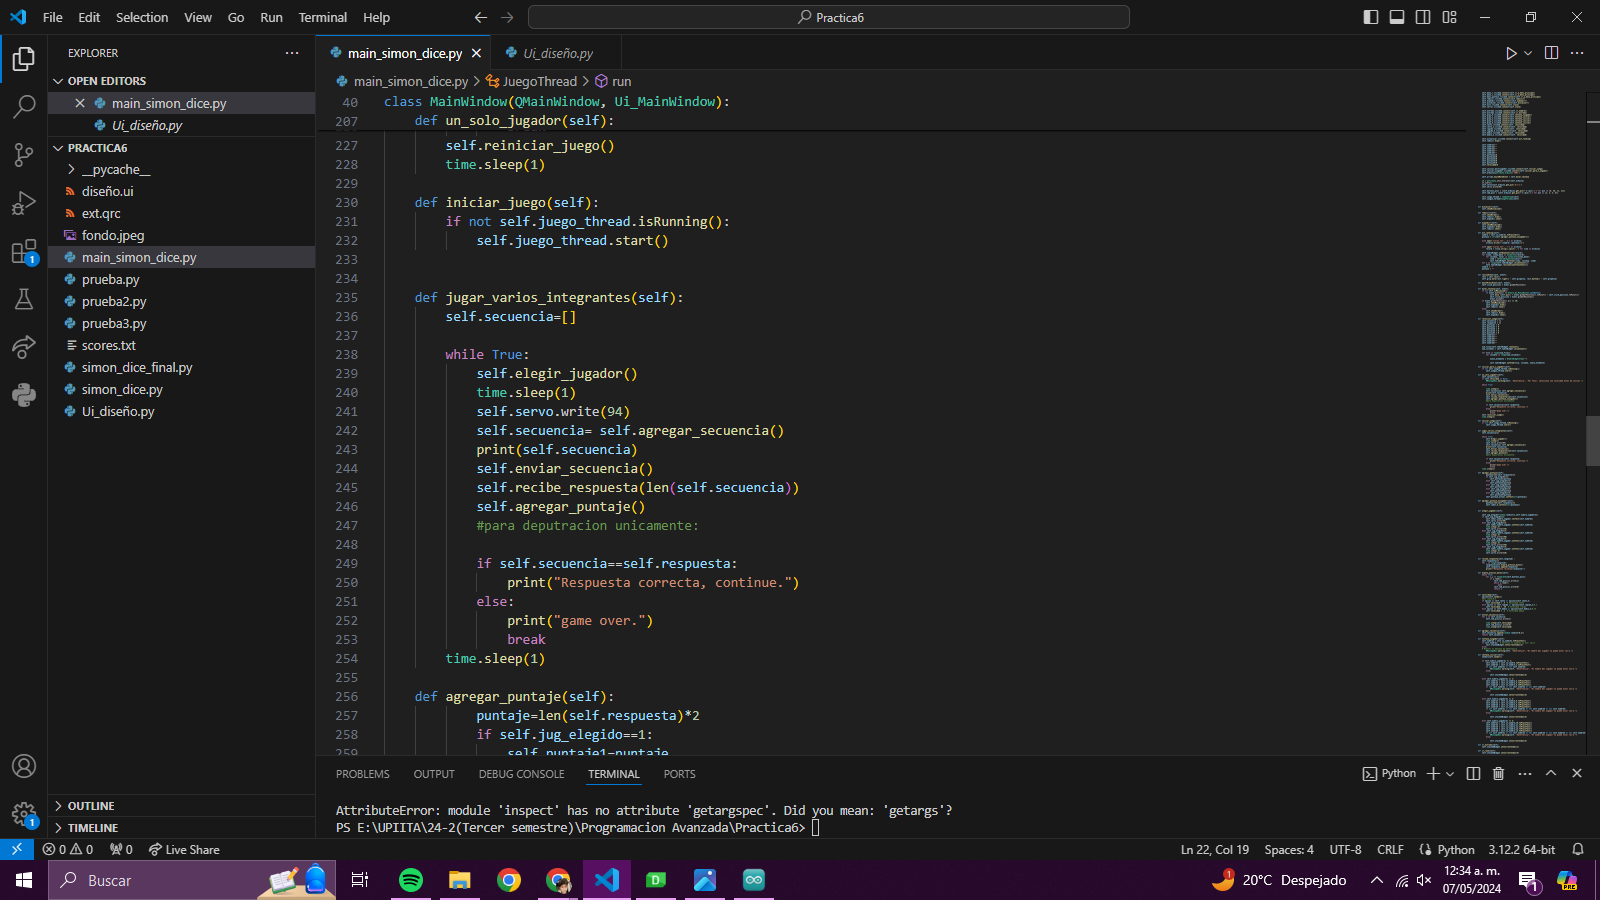
\includegraphics[width=1\textwidth]{Captura de pantalla (771).png}
    
\end{figure}

{\Large La función `jugarvariosintegrantes` ejecuta el juego para múltiples jugadores, donde se elige un jugador aleatorio, se genera una secuencia de juego, se envía al jugador, se espera su respuesta, se actualiza el puntaje del jugador y se verifica si la respuesta es correcta. Si la respuesta es incorrecta, el juego se detiene y se reinicia.

La función `agregarpuntaje` asigna el puntaje correspondiente al jugador seleccionado y lo muestra en la interfaz.

La función `agregarpuntajeunjugador` asigna el puntaje al jugador único y lo muestra en la interfaz.

}


\newpage
\begin{figure}[h]
    \centering
    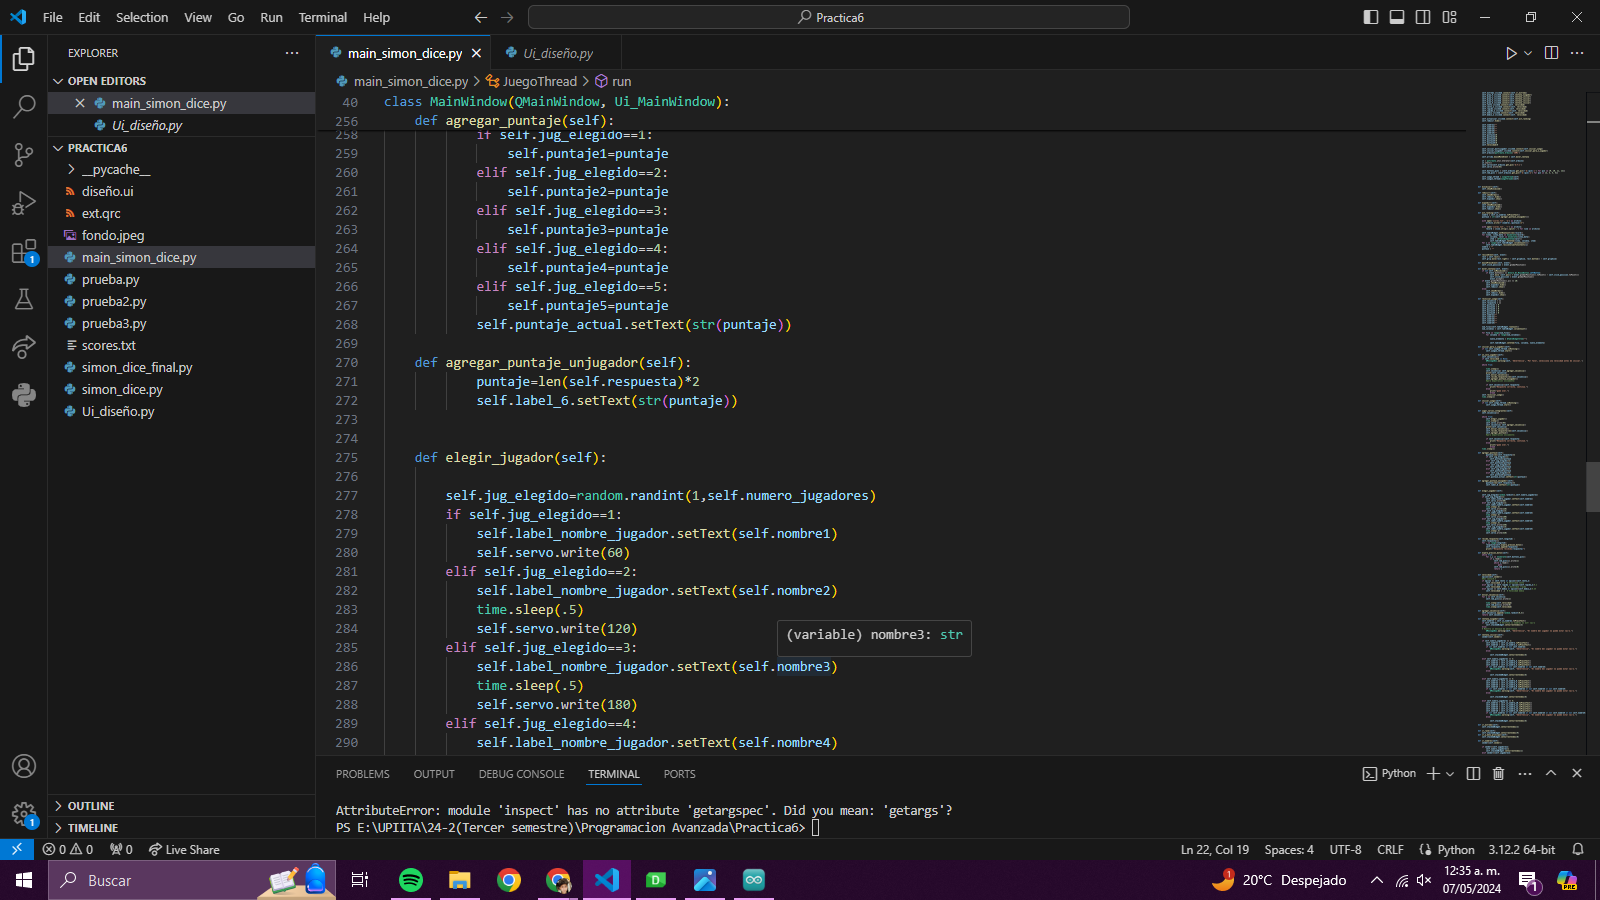
\includegraphics[width=1\textwidth]{Captura de pantalla (772).png}
    
\end{figure}

{\Large La función `elegirjugador` elige aleatoriamente a uno de los jugadores disponibles y actualiza la interfaz para mostrar su nombre. Además, envía una señal al Arduino para controlar un servo que indica al jugador seleccionado. El servo se mueve a diferentes ángulos según el jugador elegido, lo que podría estar relacionado con algún tipo de indicador físico en el juego.

}

\newpage
\begin{figure}[h]
    \centering
    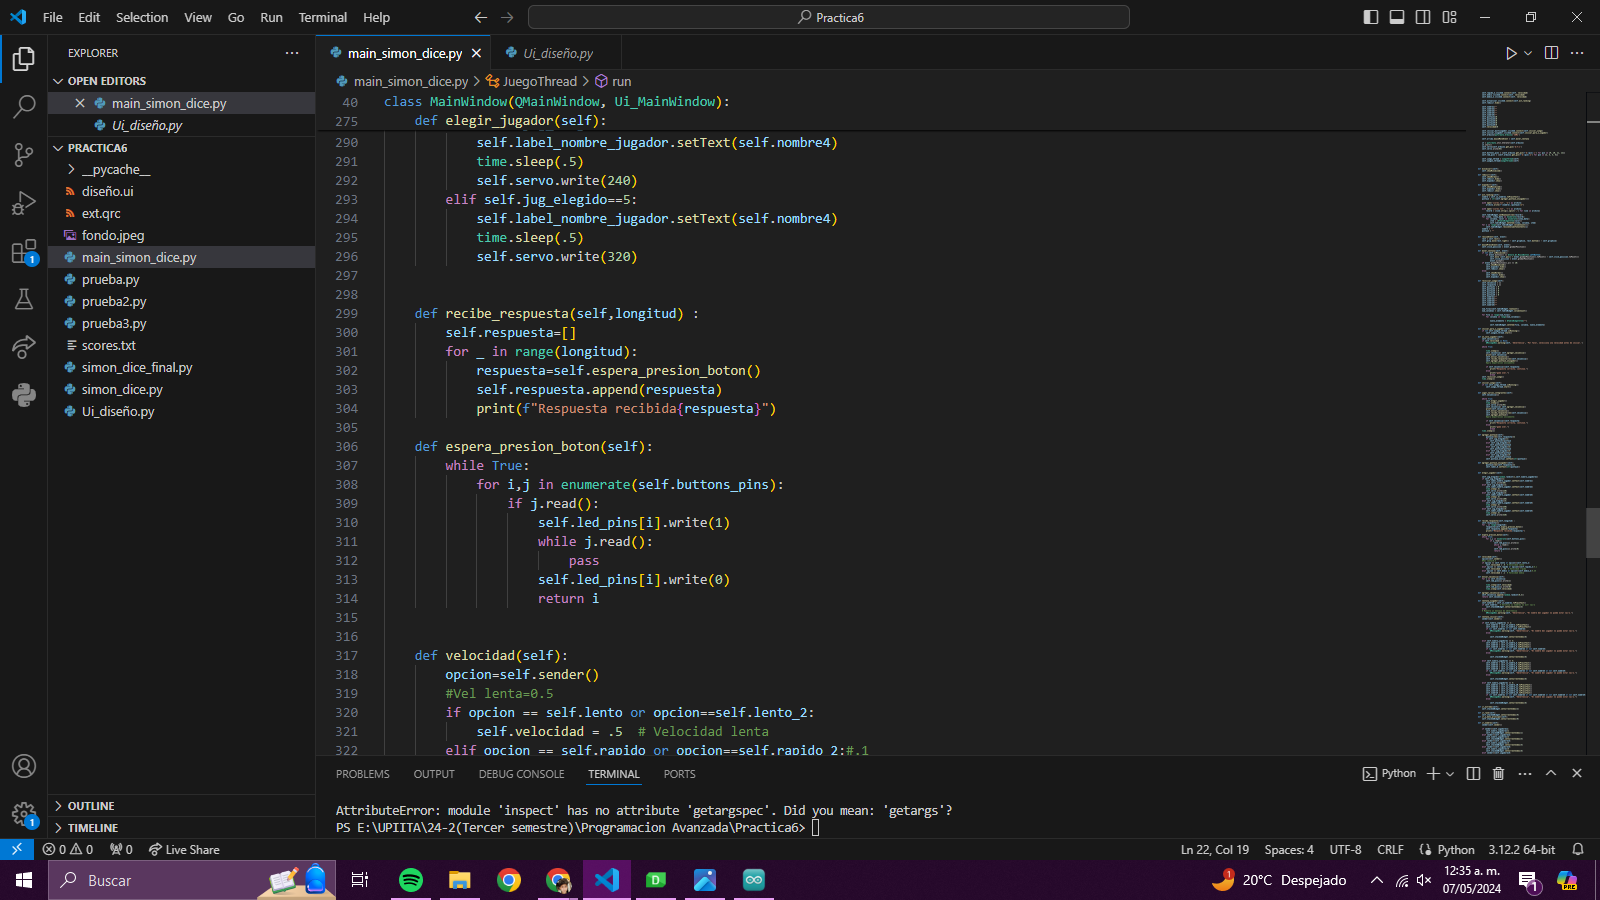
\includegraphics[width=1\textwidth]{Captura de pantalla (773).png}
    
\end{figure}

{\Large La función `reciberespuesta` espera y registra la respuesta del jugador presionando los botones. Utiliza la función `esperapresionboton` para esperar hasta que un botón sea presionado y luego registra el índice del botón presionado. Mientras tanto, enciende el LED correspondiente al botón presionado durante la espera. Una vez que se presiona un botón, el LED correspondiente se apaga y se devuelve el índice del botón presionado. Esto permite registrar la secuencia de botones presionados como respuesta del jugador.

}

\newpage
\begin{figure}[h]
    \centering
    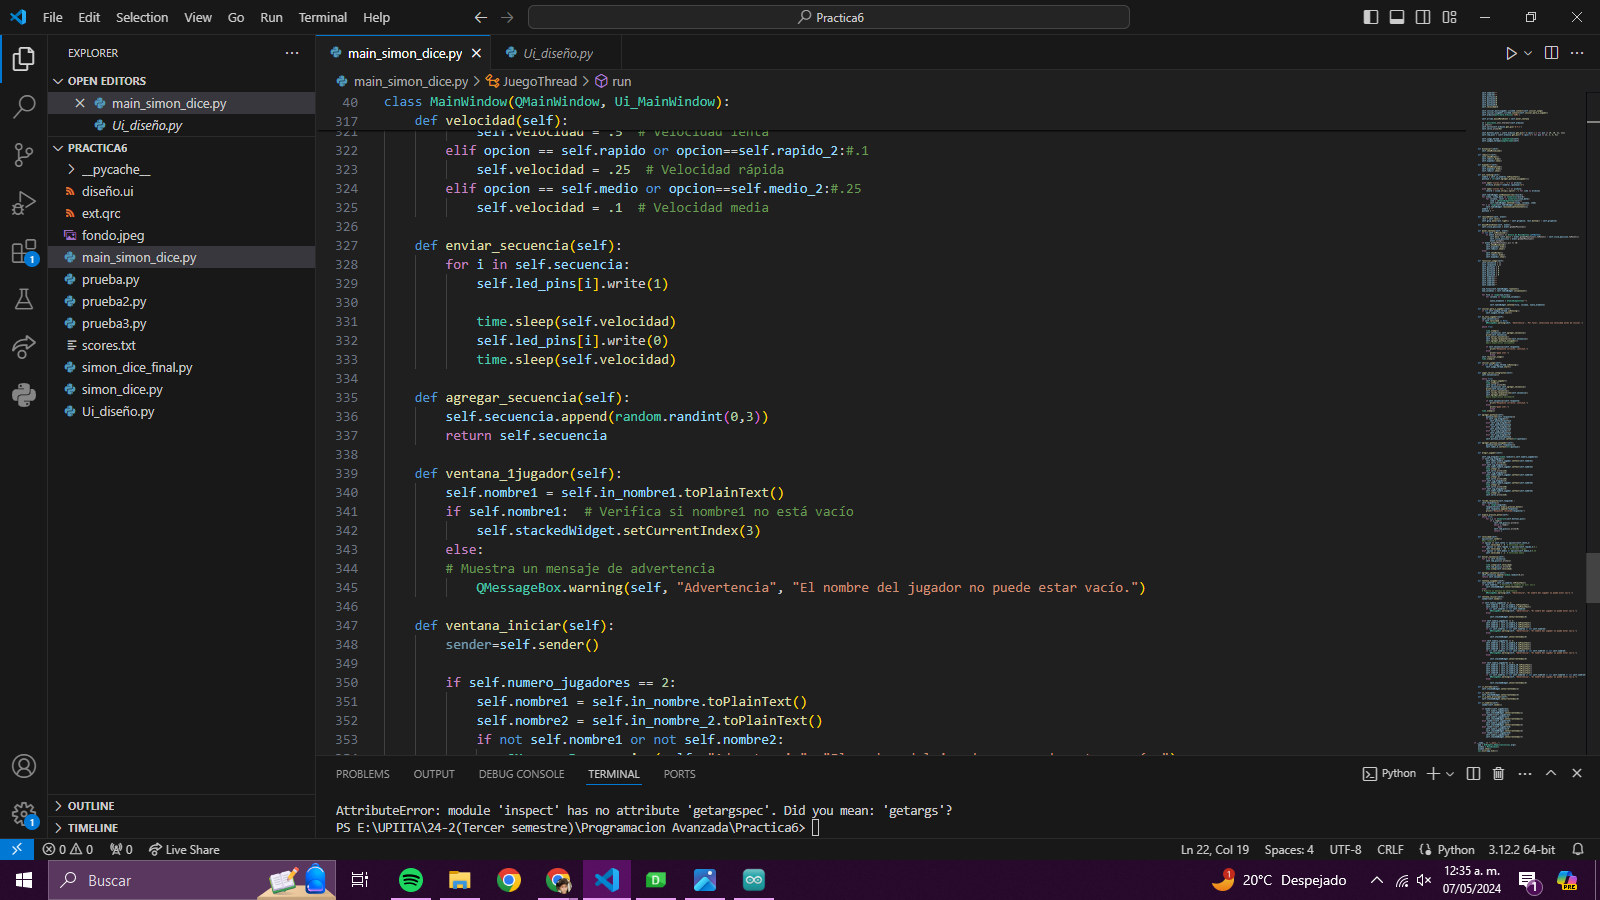
\includegraphics[width=1\textwidth]{Captura de pantalla (774).png}
    
\end{figure}

{\Large 

}

\newpage
\begin{figure}[h]
    \centering
    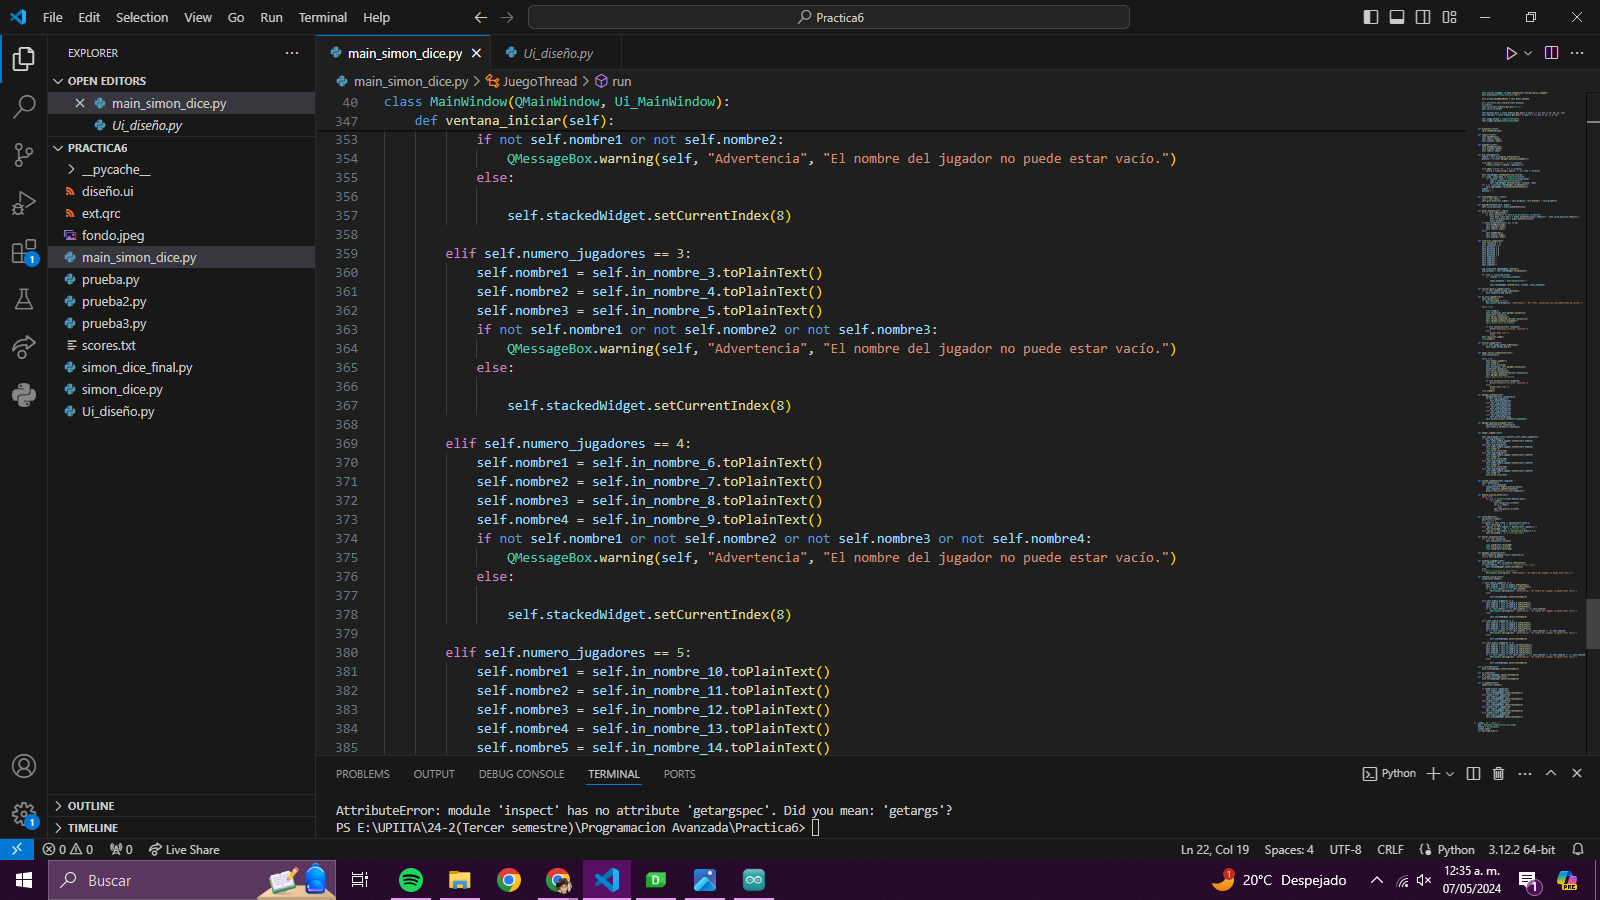
\includegraphics[width=1\textwidth]{Captura de pantalla (775).png}
    
\end{figure}

{\Large La función `velocidad` ajusta la velocidad del juego según la opción seleccionada por el usuario. Luego, la función `enviarsecuencia` enciende y apaga los LEDs correspondientes a la secuencia generada, con una pausa de tiempo determinada por la velocidad. `agregarsecuencia` genera una nueva secuencia de botones aleatorios.

Las funciones `ventana1jugador` y `ventanainiciar` manejan el flujo de la interfaz de usuario para iniciar el juego con uno o varios jugadores, respectivamente. Verifican si se ha ingresado el nombre del jugador y muestran un mensaje de advertencia si está vacío. Dependiendo del número de jugadores seleccionados, establecen el índice actual de la pila de widgets para avanzar en la interfaz de usuario.

}

\newpage
\begin{figure}[h]
    \centering
    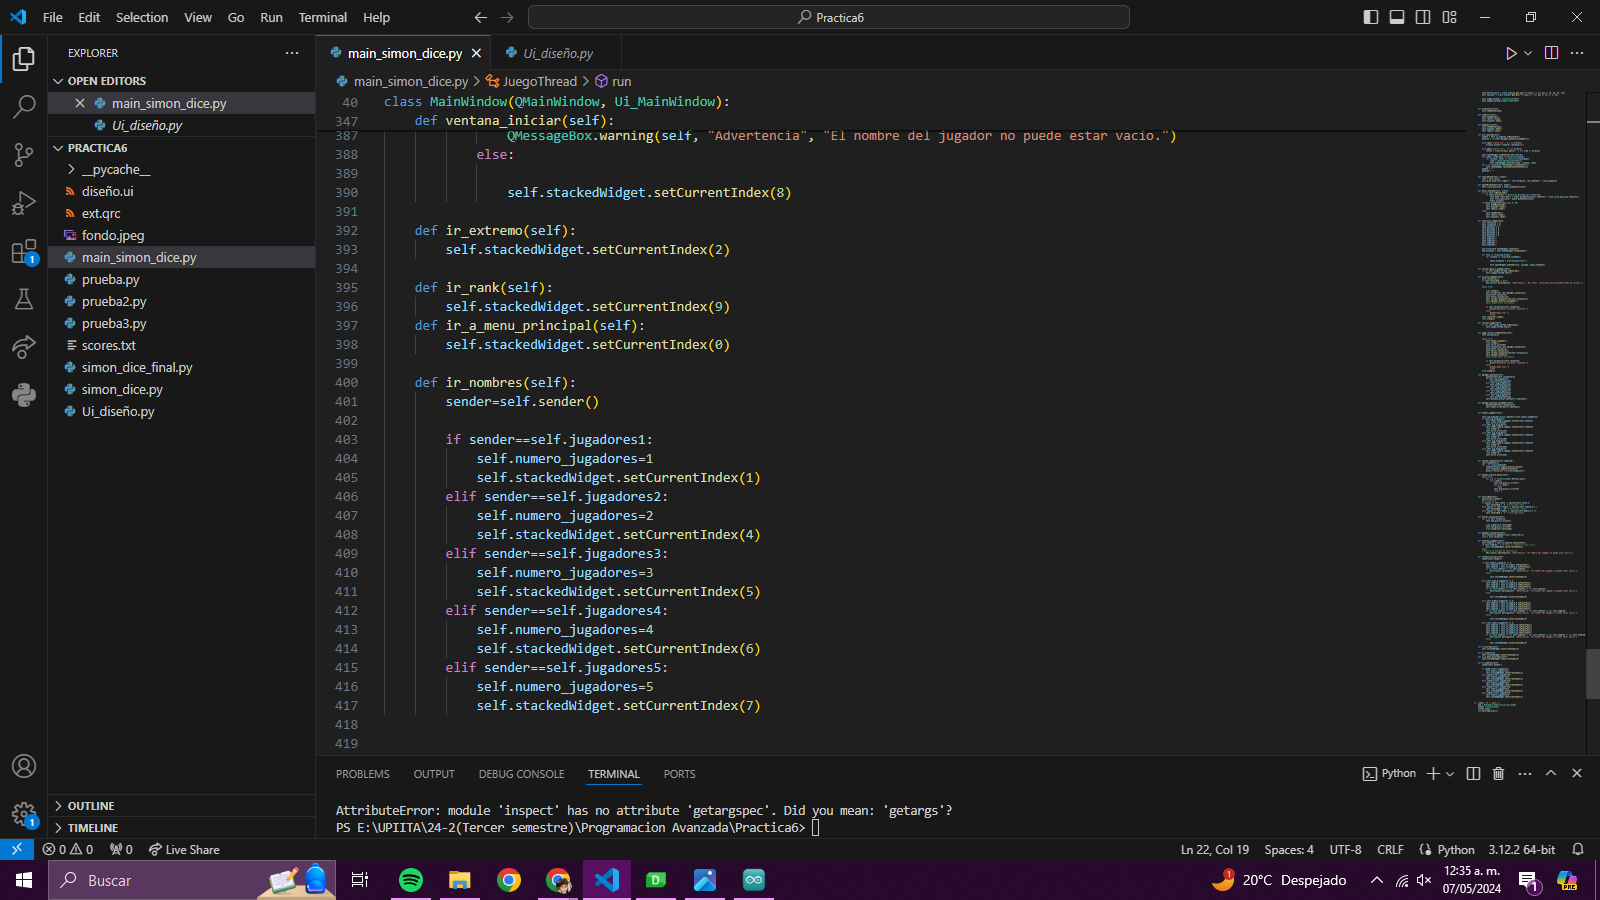
\includegraphics[width=1\textwidth]{Captura de pantalla (776).png}
    
\end{figure}

{\Large Las funciones `irextremo`, `irrank` e `iramenuprincipal` cambian el índice actual de la pila de widgets para redirigir la interfaz de usuario a diferentes pantallas: la pantalla de juego extremo, la pantalla de ranking y la pantalla del menú principal, respectivamente.

La función `irnombres` determina el número de jugadores seleccionados según el botón de jugador presionado y redirige la interfaz de usuario a la pantalla correspondiente para que los jugadores ingresen sus nombres.

}





\newpage
\subsection*{\huge Ejecución}

{\Large\\ Cuando ejecutamos nuestro codigo, nos parece la pantalla principal de simon, y se despleiga como se indico, todo aqui depende de la interaccion que se tanga con el usuario

}

\vspace{0.2cm}
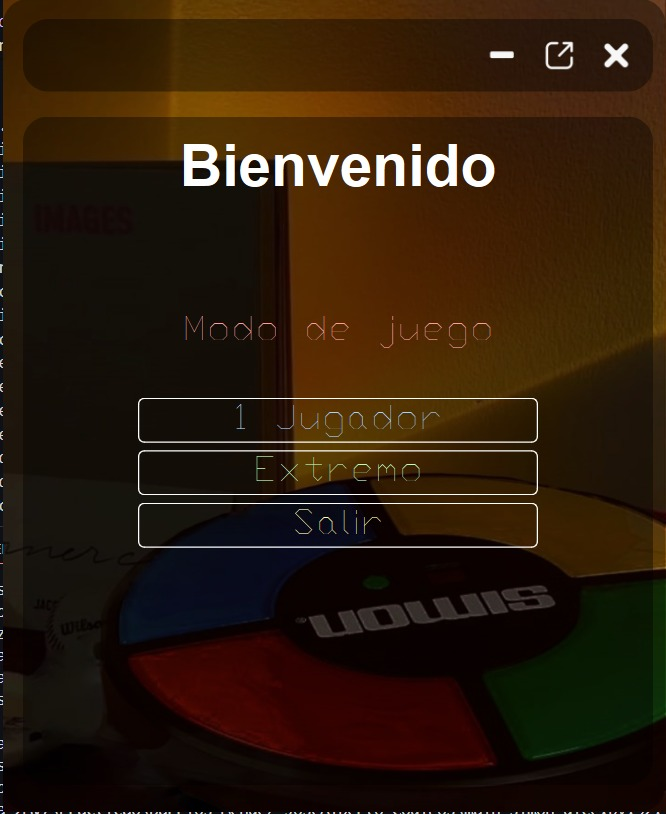
\includegraphics[width=0.5\linewidth]{cbdf35fc-d1bb-4aa4-8690-dcb82a1c29b8.jpg}
{\Large \\Podemos observar las conexiones del arduino y la conexion del puerto serial, ya que sin este no puede cargar el programa ya que se le asigno una conexion serial

}


\vspace{0.2cm}


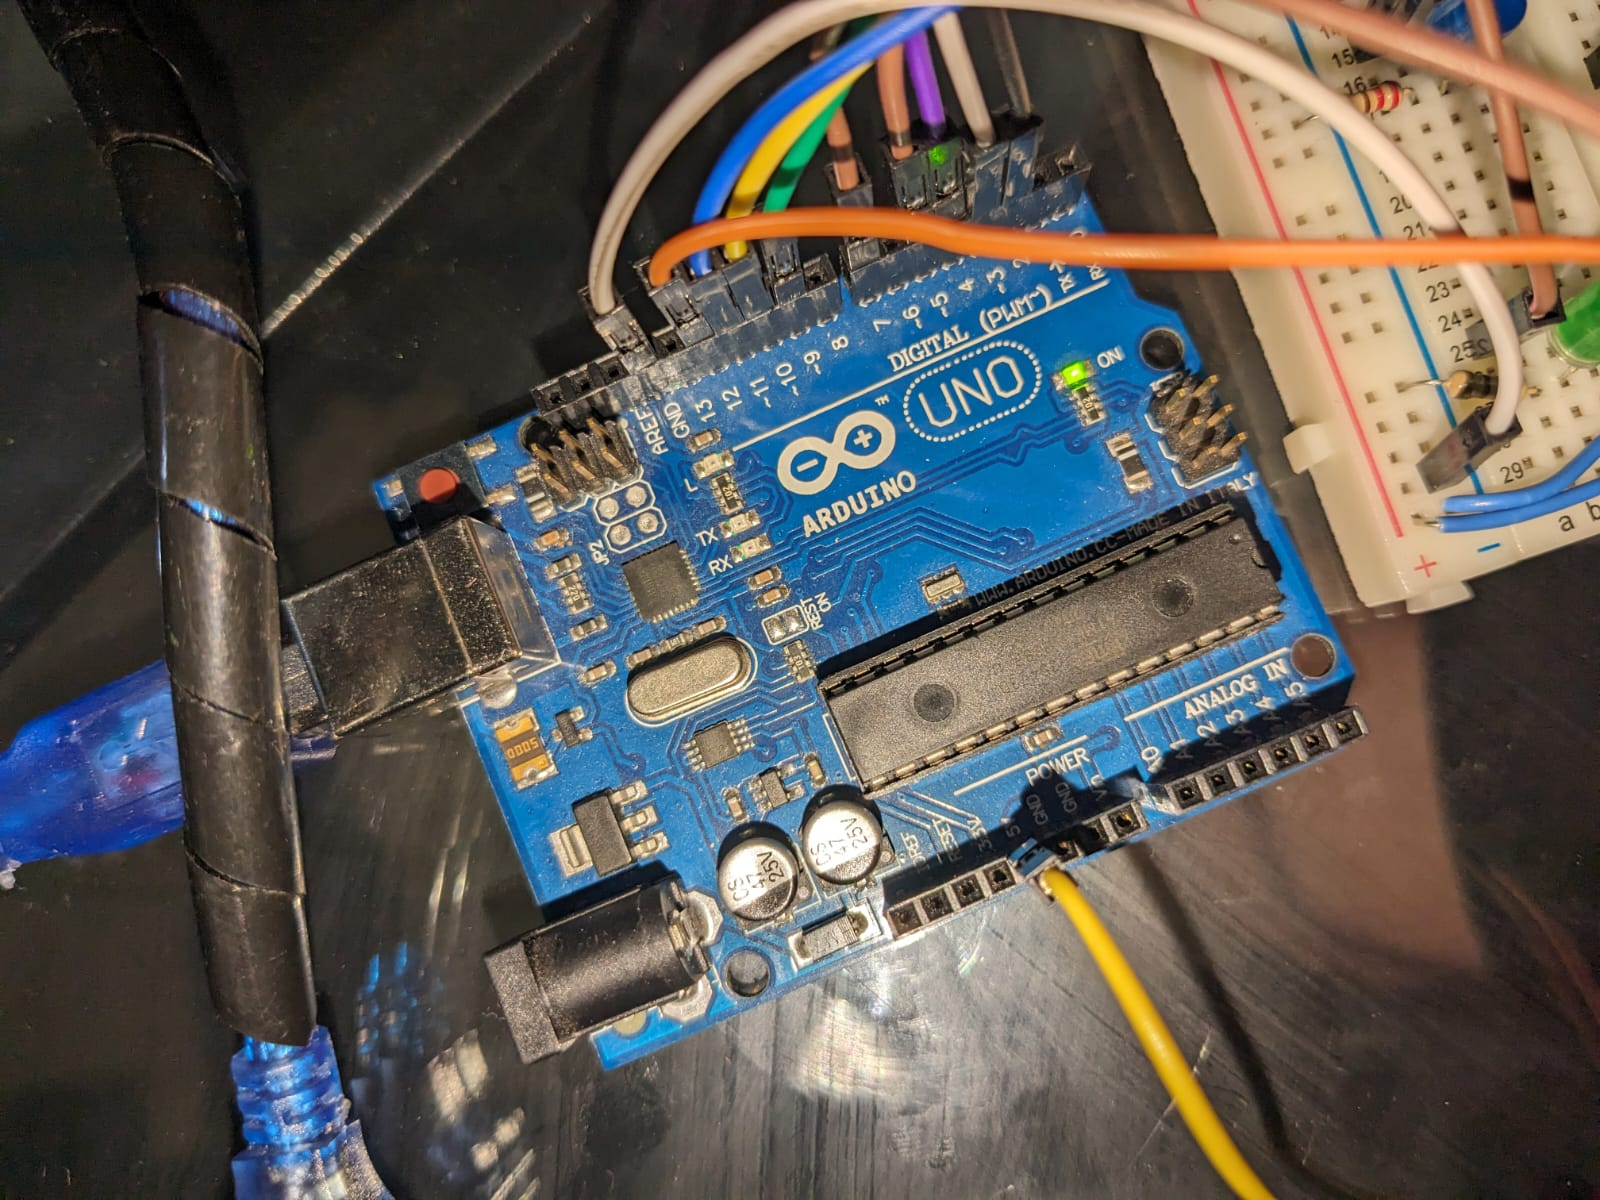
\includegraphics[width=0.5\linewidth]{f7e61b87-70d0-4296-bf4a-1963941b228b.jpg}

\vspace{0.2cm}




\newpage


\vspace{0.2cm}
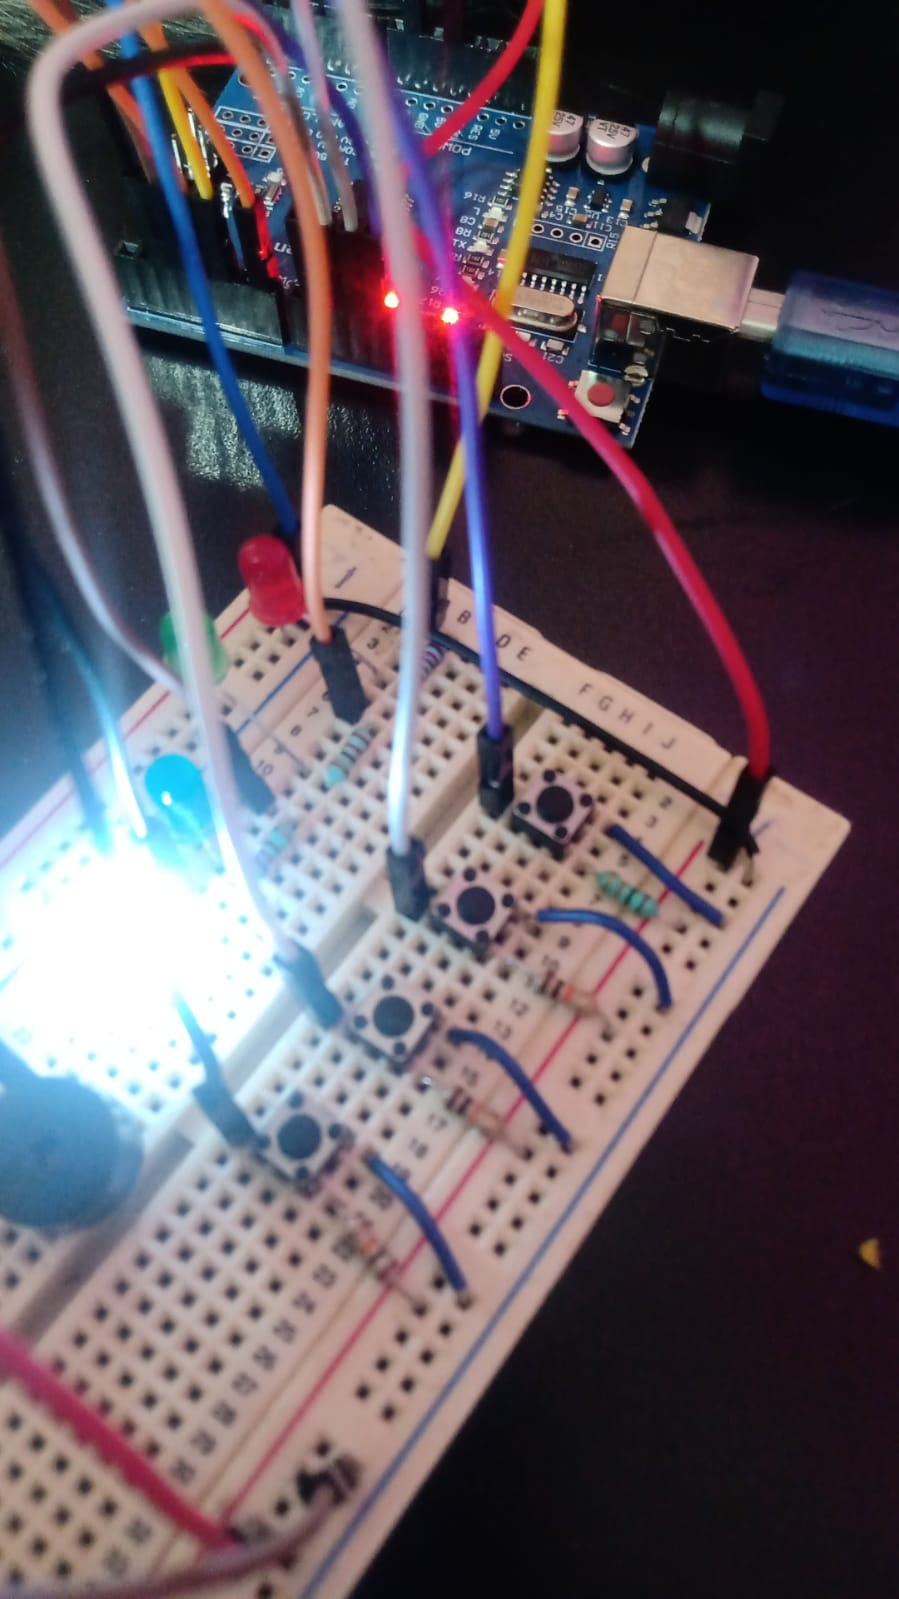
\includegraphics[width=0.5\linewidth]{1371cd04-dfd8-4b58-b8c8-869f93134617.jpg}

\vspace{0.2cm}


{\Large Finalmente observamos el encendido y apagado de los leds de la secuencia que se mando a imprimir...
}

\newpage



\section*{Conclusiones}

{\Large Usar una interfaz gráfica de usuario (GUI) en Python junto con Arduino ha sido una experiencia fascinante para nosotros. Ha ampliado significativamente las posibilidades de lo que podemos lograr con nuestros proyectos, agregando una capa visual y de interacción que antes no teníamos.\\

La interactividad mejorada es uno de los aspectos más destacados. La combinación de Python y Arduino nos ha permitido crear interfaces de usuario que responden a la entrada del usuario y a las lecturas de sensores en tiempo real. Esto ha mejorado enormemente la experiencia de usuario y ha hecho que nuestros proyectos sean más atractivos y fáciles de usar.\\

Además, la capacidad de visualizar datos recopilados por los sensores de Arduino en una GUI ha sido muy útil. Podemos representar gráficamente los datos de manera clara y comprensible, lo que facilita el monitoreo y análisis de los mismos, especialmente en proyectos relacionados con la monitorización del medio ambiente o la domótica.\\

La posibilidad de control remoto y automatización es otro aspecto importante. Integrar una GUI con Arduino nos ha permitido controlar dispositivos físicos y sistemas embebidos de forma remota a través de la red. Esto ha abierto la puerta a la automatización de tareas y procesos, mejorando la eficiencia y comodidad en una variedad de situaciones.\\

El prototipado rápido también se ha beneficiado enormemente de esta combinación. Podemos crear interfaces de usuario rápidamente para probar y demostrar conceptos antes de invertir tiempo en el desarrollo de una solución completa. Esto ha sido invaluable para iterar y refinar nuestras ideas de manera rápida y efectiva.\\

En términos de flexibilidad y escalabilidad, Python y Arduino son herramientas altamente versátiles. Esta combinación nos permite adaptar nuestros proyectos a una amplia variedad de aplicaciones y requisitos, ya sea trabajando en un proyecto simple o en uno más complejo.\\

}

\vspace{3\baselineskip}


\bibliographystyle{apalike}

\begin{thebibliography}{9} 

\bibitem  Editronikx. (2022, June 5). comunicación y control con python y arduino mediante pyserial y visual code studio [Video]. YouTube. https://www.youtube.com/watch?v=RuCE6PLyym0 

\bibitem  Julian Ruiz. (2021, January 14). ✅Como conectar PYTHON con ARDUINO �� [2022] | Julian Ruiz [Video]. YouTube. https://www.youtube.com/watch?v=fCuFDW1RoxI

\bibitem  Network Warriors. (2021, September 27). Comunicación Python - Arduino  (Pycharm) pyserial || Enviar y Recibir Datos [Video]. YouTube. https://www.youtube.com/watch?v=_DMFDjNYNVI


\end{thebibliography}

\end{document}


